%% -----------------------------------------------------------------
%% This file uses UTF-8 encoding
%%
%% For compilation use following command:
%% latexmk -pdf -pvc -bibtex thesis
%%
%% -----------------------------------------------------------------
%%                                     _     _      
%%      _ __  _ __ ___  __ _ _ __ ___ | |__ | | ___ 
%%     | '_ \| '__/ _ \/ _` | '_ ` _ \| '_ \| |/ _ \
%%     | |_) | | |  __/ (_| | | | | | | |_) | |  __/
%%     | .__/|_|  \___|\__,_|_| |_| |_|_.__/|_|\___|
%%     |_|                                          
%%
%% -----------------------------------------------------------------
\documentclass{kithesis}

% Additional packages
\usepackage[main=slovak,english]{babel}
\usepackage{listings} 
\usepackage{amsmath} 
\usepackage{multirow} 
\usepackage{booktabs}
\usepackage{indentfirst}
\usepackage{dirtree}
\usepackage{hyperref}
  % for source code
% Listings settings
% See for details: https://en.wikibooks.org/wiki/LaTeX/Source_Code_Listings
\lstset{              % nastavení
	%	Definice jazyka použitého ve výpisech
	%    language=[LaTeX]{TeX},	% LaTeX
	%	language={Matlab},		% Matlab
	language={C},           % jazyk C
	basicstyle=\ttfamily,	% definice základního stylu písma
	tabsize=2,			% definice velikosti tabulátoru
	mathescape=<true>,
	inputencoding=utf8,         % pro soubory uložené v kódování UTF-8
	columns=fixed,  %fixed nebo flexible,
	fontadjust=true %licovani sloupcu
	extendedchars=true,
	literate=%  definice symbolů s diakritikou
	{á}{{\'a}}1
	{č}{{\v{c}}}1
	{ď}{{\v{d}}}1
	{é}{{\'e}}1
	{ě}{{\v{e}}}1
	{í}{{\'i}}1
	{ň}{{\v{n}}}1
	{ó}{{\'o}}1
	{ř}{{\v{r}}}1
	{š}{{\v{s}}}1
	{ť}{{\v{t}}}1
	{ú}{{\'u}}1
	{ů}{{\r{u}}}1
	{ý}{{\'y}}1
	{ž}{{\v{z}}}1
	{Á}{{\'A}}1
	{Č}{{\v{C}}}1
	{Ď}{{\v{D}}}1
	{É}{{\'E}}1
	{Ě}{{\v{E}}}1
	{Í}{{\'I}}1
	{Ň}{{\v{N}}}1
	{Ó}{{\'O}}1
	{Ř}{{\v{R}}}1
	{Š}{{\v{S}}}1
	{Ť}{{\v{T}}}1
	{Ú}{{\'U}}1
	{Ů}{{\r{U}}}1
	{Ý}{{\'Y}}1
	{Ž}{{\v{Z}}}1
}
\def\lstlistingname{Zdrojový kód}
\lstset{mathescape=<true>}
% Variables 
%zadanie z maisu
%\thesisspec{figures/meno.png} 

\title{Lightweight cryptography in VPN networks \br)}{Ľahká kryptografia vo VPN sieťach\br }


\author{Bc. Marek}{Rohač}
\supervisor{prof. Ing. Miloš Drutarovský, CSc.} %veduci prace
\consultant{} %konzultant
\college{Technical University of Košice}{Technická univerzita v Košiciach} %univerzita
\faculty{Faculty of Electrical Engineering and informatics}{Fakulta elektrotechniky a informatiky} %fakulta
\department{Department of electronies and multimedia telecommunications}{Katedra elektroniky a multimediálnych telekomunikácií} %katedra
\departmentacr{DEMT}{KEMT} % skratka katedry
\thesis{Master thesis}{Diplomová práca} %typ prace
\submissiondate{ 28}{ 5}{ 2023}
\fieldofstudy{Informatika}
\studyprogramme{Počítačové siete}
%\city{Košice}
\keywords{DSVPN, Lightweight Cryptography, Linux, VPN, Windows, XOODOO}{DSVPN, Ľahká kryptografia, Linux, VPN, Windows, XOODOO}
\declaration{Vyhlasujem, že som záverečnú prácu vypracoval samostatne s použitím uvedenej odbornej literatúry.}

\abstract{english
}{slovak}


\acknowledgment{Na~tomto mieste by~som rád poďakoval svojmu vedúcemu práce \textit{prof. Ing. Milošovi Drutarovskému, CSc.} za jeho čas a odborné vedenie počas celého riešenia záverečnej práce.}

% if you want to work only on selected chapters
%\includeonly{chapters/analyza} %,chapters/synteza}
% Load acronyms
% Acronyms
% ========
%
% An acronym is a word formed from the initial letters in a phrase. 
%
% Acronym Definition Exapmle:
% ---------------------------
% \newacronym{gcd}{GCD}{Greatest Common Divisor}
% \newacronym{dry}{DRY}{Don't Repeat Yourself}
%
% Usage:
% ------
% You can use these three options:
% 
% \acrlong{}  
%   Displays the phrase which the acronyms stands for. Put the label of the acronym inside the braces. In the example, \acrlong{gcd} prints Greatest Common Divisor. 
%
% \acrshort{} 
%   Prints the acronym whose label is passed as parameter. For instance, \acrshort{gcd} renders as GCD. 
%
% \acrfull{ } 
%   Prints both, the acronym and its definition. In the example the output of \acrfull{dry} is Don't Repeat Yourself (DRY). 
% 
% For more information see:
% -------------------------
% * https://www.sharelatex.com/learn/Glossaries 
% * https://en.wikibooks.org/wiki/LaTeX/Glossary
%


\newacronym{vpn}{VPN}{Virtual Private Network}
\newacronym{vm}{VM}{Virtual Machine}
\newacronym{vb}{VB}{Virtual Box}
\newacronym{lts}{LTS}{Long Term Support}
\newacronym{os}{OS}{Operating System}
\newacronym{tcp}{TCP}{Transmission Control Protocol}
\newacronym{oss}{OSS}{Operating System Server}
\newacronym{osc}{OSC}{Operating System Client}
\newacronym{ip}{IP}{Internet Protocol}
\newacronym{ftp}{FTP}{File Transfer Protocol}
\newacronym{tls}{TLS}{Transport Layer Security}
\newacronym{ssl}{SSL}{Secure Socket Layers}
\newacronym{gw}{GW}{GateWay}
\newacronym{fw}{FW}{FireWall}
\newacronym{pdv}{PDV}{Packet Delay Variation}
\newacronym{aes}{AES}{Advanced Encryption Standard}
\newacronym{fskd}{FSKD}{Full-State Keyed Duplex}
\newacronym{tcpip}{TCP/IP}{Transmission Control Protocol/Internet Protocol reference model}
\newacronym{osi}{OSI}{Open Systems Interconnection reference model}
\newacronym{http}{HTTP}{HyperText Transfer Protocol}
\newacronym{smtp}{SMTP}{Simple Mail Transfer Protocol}
\newacronym{udp}{UDP}{User Datagram Protocol}
\newacronym{l}{L}{Layer}






%% -----------------------------------------------------------------
%%          _                                       _   
%%       __| | ___   ___ _   _ _ __ ___   ___ _ __ | |_ 
%%      / _` |/ _ \ / __| | | | '_ ` _ \ / _ \ '_ \| __|
%%     | (_| | (_) | (__| |_| | | | | | |  __/ | | | |_ 
%%      \__,_|\___/ \___|\__,_|_| |_| |_|\___|_| |_|\__|
%%                                                      
%% -----------------------------------------------------------------

\begin{document}
%% Title page, abstract, declaration etc.:
\frontmatter{}

%% List of code listings, if you are using package minted
%\renewcommand\lstlistlistingname{Zoznam zdrojových kódov}
%\lstlistoflistings{}

\pagenumbering{arabic}

%% Chapters
% !TEX root = ../thesis.tex

\chaptermark{Úvod}
\phantomsection
\addcontentsline{toc}{chapter}{Úvod}

\chapter*{Úvod}
\blindtext
\acrshort{vpn}
\cite{book}



% !TEX root = ../thesis.tex

\chapter{Virtual Private Network -- VPN}\label{1}
Virtuálna privátna sieť (ďalej \textbf{\acrshort{vpn}}) je jeden zo spôsobov prepojenia zariadení, tak že internetová komunikácia medzi nimi je privátna, resp. zabezpečená aj v prípade používania nezabezpečenej, verejnej siete. Bezpečnosť spojenia je docielená pomocou kryptografických protokolov v tuneli, ktorý VPN vytvára. 
Táto technológia patrí aktuálne k najpoužívanejším spôsobom pripojenia sa medzi 2 rôznymi internetovými doménami. Najčastejší výskyt je možné sledovať v korporačnom prostredí, pričom cieľom je rozšírenie možností bezpečného pripojenia sa k firemnej sieti. Vzhľadom na firemné tajomstvá je nutné aby bolo takéto spojenie bezpečné a zamestnanci sa mohli pripojiť z rôznych miest. Vďaka uvedeným vlastnostiam je následne možná aj práca z~domu (z~ang. \textit{Home office}), ktorá môže byť benefitom pre obe strany. Ukážka použitia VPN je znázornená pomocou \ref{vpndemo}. 
\begin{figure}[!ht]
	\centering
	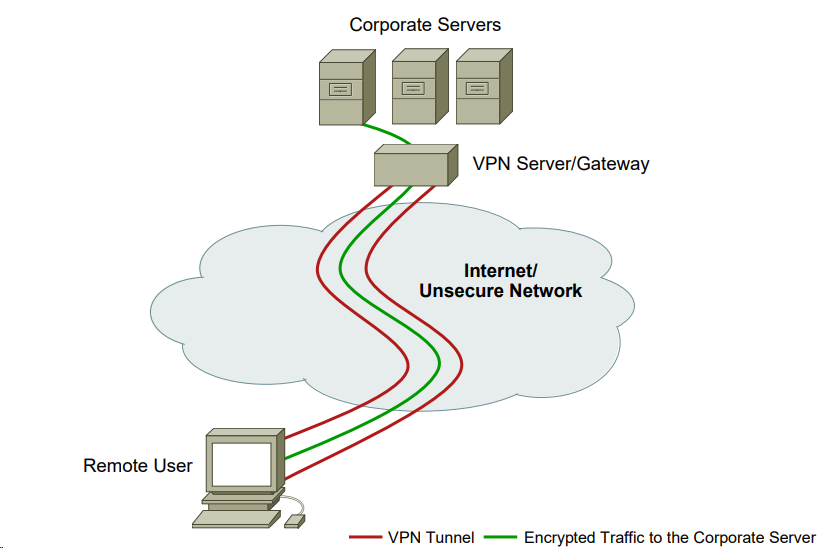
\includegraphics[width=.9\textwidth]{figures/VPNdemo}
	\caption{Ukážka typického VPN pripojenia}
	\label{vpndemo}
\end{figure}

\section{Rozdelenie VPN}
\cite{divvpn}, \cite{ciscovpn}

\section{Protokol riadenia prenosu -- \acrshort{tcp}}
Protokol riadenia prenosu (z ang. \textit{Transmission Control Protocol}, ďalej \acrshort{tcp}) je komunikačný protokol orientovaný na nadviazanie a udržanie sieťového spojenia medzi zariadeniami. Môže byť použitý pri úlohe príjímateľa aj odosielateľa (z ang. \textit{full-duplex}). Úlohou je spoľahlivý prenos dát medzi komunikantmi. Odoslanie a príjem dát je v rovnakom poradí. Protokol zároveň obsahuje mechanizmy na kontrolu výskytu chýb. 

Na začiatku 21. storočia je 95\% paketov používaných na internete TCP. Bežné aplikácie používajúce TCP sú webové (HTTP/HTTPS protokoly), slúžiace na e-mailovú komunikáciu (SMTP/POP3/IMAP) a prenos súborov (z ang. \textit{File Transfer Protocol -- \acrshort{ftp}}). Minimálna dĺžka hlavičky TCP je 20 bajtov a maximálna dĺžka 60 bajtov. Po pridaní údajov TCP hlavičky k prenášaným dátam, vzniká tzv. \textit{segment}. TCP je použitý s internetovým protokolom (ďalej \acrshort{ip}) Z uvedeného dôvodu sa preto často stretávame s označením TCP/IP. Dôležité je však poznamenať, že sa jedná o jeden a ten istý TCP protokol. 

V súvislosti s TCP/IP sa používateľ môže stretnúť s modelom. Ten je zobrazený pomocou schémy \ref{tcpipprot}. V uvedenej schéme sú znázornené aj niektoré z protokolov, ktoré ja na jednotlivých vrstvách používajú.

\begin{figure}[!ht]
	\centering
	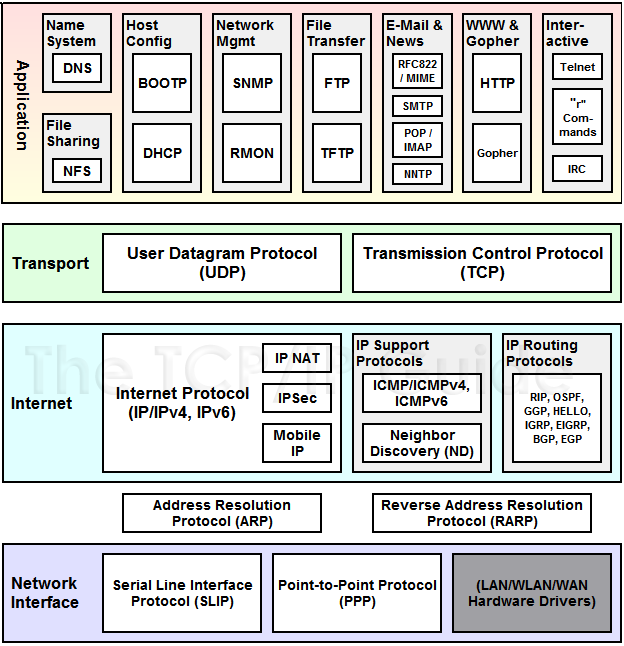
\includegraphics[width=0.9\textwidth]{figures/tcpipprot}
	\caption{Schéma TCP/IP modelu s niektorými protokolmi}
	\label{tcpipprot}
\end{figure}

V súčasnosti je možne TCP protokol implementovať softvérovo aj hardvérovo. Pri prvom z uvedených je problémom závislosť na OS a následne aj vysoká vyťaženosť procesora pri príprave a spracovaní dát. Pri hardvérovom riešení je výhodou optimalizácia a implementácia bez potreby dodatočnej úpravy OS. Hardvérové implementácie sa realizujú pomocou koprocesorov umiestnených vo vnútri procesora. Následkom toho môžeme dnes bežne pozorovať umiestnenie spomenutých zariadení na našich zariadeniach.

Podrobnejšie informácie o TCP protokole je možné nájsť na \cite{tcp2}. V uvedenej publikácií sa nachádza opis TCP hlavičky, metódy nadviazania a ukončenia spojenia. Obdobne je spomenuté ako dochádza k prenosu dát pomocou sekvenčných čísel. Ak má používateľ nejasnosti v fungovaní TCP protokolu, odporúča sa danú publikáciu prečítať.

\section{Kryptografické zabezpečenie protokolov}
TCP protokol sam o sebe nezabezpečí dáta, ku ktorým sa pridáva TCP hlavička. Dôsledkom toho vznikli viacere protokoly slúžiace na autentizované šifrovanie dát. Najznámejší je protokol zabezpečenia prenosu -- \acrshort{tls} a IPSec.
\subsection{Transport Layer Security -- TLS}
Zabezpečenie dát bolo prvotne vykonávané pomocou protokolu \textit{Secure Sockets Layer} -- \acrshort{ssl}. Tento spôsob používa certifikáty na odšifrovanie dát. SSL malo od svojho vytvorenia dlhý vývoj, ktorý smeroval až k doteraz najpoužívanejšiemu TLS vo verzii 1.3. Inými slovami, TLS protokol je nástupca SSL pričom obsahuje rôzne úpravy a vylepšenia najmä z hľadiska rýchlosti. Zároveň sa v dnešnej dobe neodporúča používanie SSL protokolu. Dôsledkom optimalizácií je, že klienta komunikujúci so serverom cez HTTPS protokol s TLS 1.3 je rýchlejší ako v prípade použitia nešifrovaného HTTP variantu. 

TLS pracuje niekde na pomedzi aplikačnej a transportnej vrstvy. Spôsob spracovania dát je zobrazený pomocou schémy \ref{ssl} s SSL operáciami, prebratej z \cite{biks}. 
\begin{figure}[!ht]
	\centering
	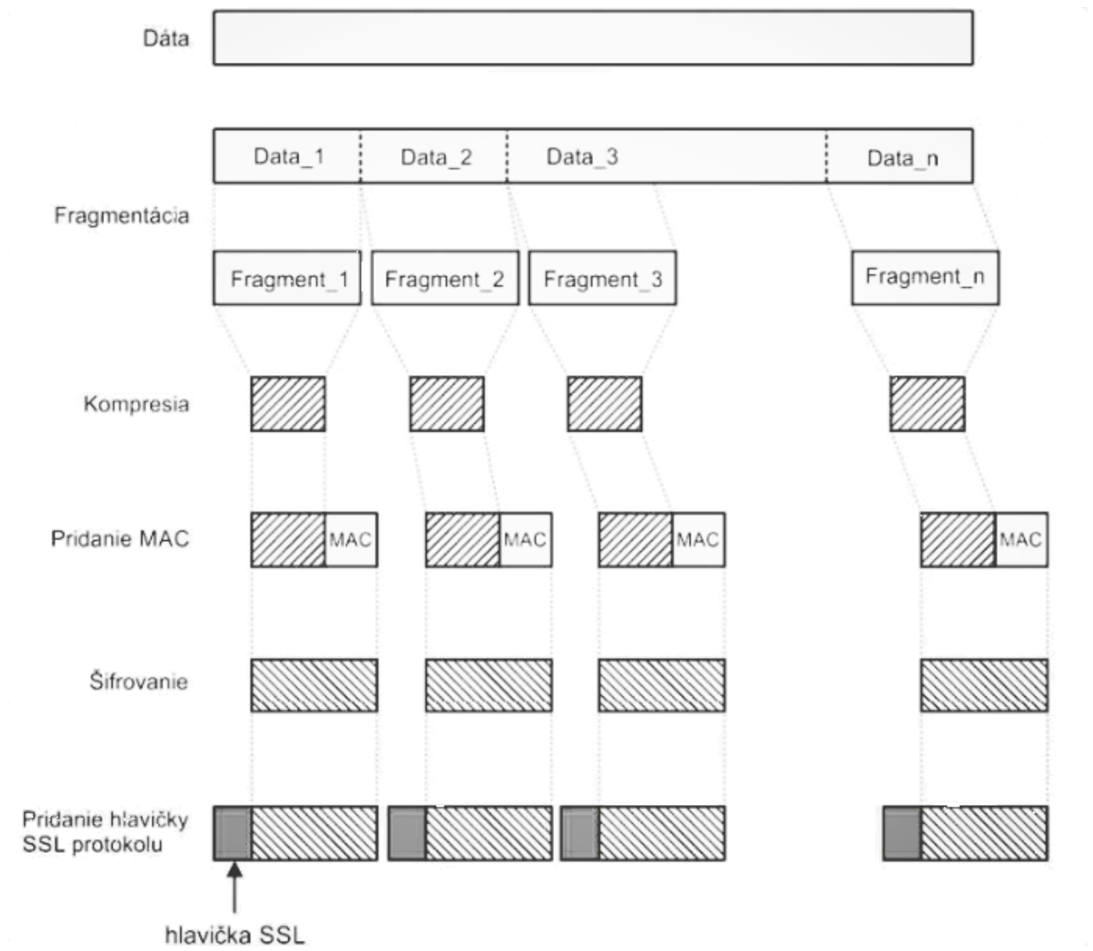
\includegraphics[width=0.7\linewidth]{figures/ssl}
	\caption{Prehľad operácií v SSL protokole}
	\label{ssl}
\end{figure}

Viac informácií o TLS protokole, jednotlivých verziách a optimalizáciách je možné nájsť na \cite{tls}. 

\subsection{Internet Protocol Security  -- IPSec}
Ochrana medzi transportnou a sietovou vrstvou TCL/IP.
Nabudúce. \cite{biks}
\chapter{Kryptografia vo VPN}\label{krypto}
Cieľom kryptografických blokov je utajiť správu pri jej ceste z bodu A do B. Teda od odosielateľa (tvorcu) správy, až k jej príjimateľovi. Dôsledkom tohto úkonu dochádza k zabezpečeniu 3 hlavných úloh kryptografie:
\begin{itemize}
	\item \textbf{Ochrana osobných údajov} (dôvernosť) -- z ang. \textit{Data Privacy}, 
	\item \textbf{Autenticita údajov} (prišla z miesta, kde sa uvádza)  -- z ang. \textit{Data Authenticity},
	\item \textbf{Integrita údajov} (nebola upravovaná na ceste)  -- z ang. \textit{Data Integrity}.
\end{itemize}

 Prvý z uvedených bodov je najčastejšie žiadaným a známym cieľom. Odosielateľ správy zašifruje jej obsah pomocou použitia niektorého z šifrovacích algoritmov, kryptografického kľúča a následne správu odošle. Na druhej strane, príjmateľ, musí použiť komplementárny dešifrovací algoritmus s prislúchajúcim kľúčom. Ktokoľvek kto sa dostane medzi týchto komunikantov, k takto preposielanej správe, z nej nedokáže obsahovo nič zistiť, v istom časovom období. 
 
 Dôsledkom týchto faktov je jasné, že komunikanti musia mať jasne definovaný použitý algoritmus. Zároveň je nutné aby došlo k výmene kryptografických kľúčov, ktoré sú pri šifrovaní a dešifrovaní aplikované. Tým sa zabezpečí aj druhá úloha -- Autenticita dát, pretože potrebné informácie budú mať len komunikanti. 
 
 V kryptografických blokoch sú taktiež aplikované algoritmy na overenie integrity správ. Ich úlohou je potvrdiť, že do obsahu správy nebolo, počas jej transportu medzi komunikantmi, nič pridané, resp. ubrané.
 
 V súčasnosti má používateľ možnosť vybrať si zo širokej ponuky kryptografických algoritmov. Medzi najznámejší patrí \acrshort{aes}  \cite{aes}, ktorý je aktuálne používaný ako štandardný kryptografický algoritmus pri počítačovej komunikácií. Detailný opis jednotlivých blokov a postupov použitých v AES-e, je obsahom rôznych knižných vydaní. Pre čitateľa preto posúvam knihu \cite{levicky}, ktorá obsahuje okrem opisu AES-u aj doležité informácie, týkajúce sa kryptografických základov.

V rámci tejto práce sme sa rozhodli opísať, v súčásnosti menej známe, algoritmy: 
\begin{itemize}
	\item XOODOO \cite{tkecak}
	\item Gimli \cite{gimli}
	\item Simpira384 \cite{simpira}
\end{itemize}  
Uvedené permutácie sú použité ako kryptografické primitívum a pri následnej tvorbe ďalších kryptografickych blokov. 

\section{Kryptografický algoritmus XOODOO a variácie} 
XOODOO je sada 384-bitových kryptografických permutácií parametrizovaných počtom kôl. Funkcia kola/rundy\footnote{z ang. \textit{round}} funguje na 12 slovách\footnote{z ang. \textit{words}} po 32 bitoch, vďaka čomu je efektívna aj na procesoroch nižšej triedy. Vytvoril ju tím Keccak, ktorý stojí za viacerými úspešnými kryptografickými algoritmami. Napríklad hashovacie funkcie z rodiny SHA-3 a iné -- \cite{kecsup}. XOODOO algoritmus vznikol po vytvorení tzv. Kravatte autentizačno-šifrovacieho algoritmu \cite{kravatte}, založené na Keccak-p permutácií \cite{keccakp}. Ten sa ukázal ako dostatočne rýchly na širokom spektre platforiem. Avšak nezapadá do kategórie tzv. ľahkej kryptografie \footnote{z ang. \textit{lightweight cryptography}}.

Tím Keccak vypracoval nové riešenie. Ním bol port medzi ich prvotným Keccak-p dizajnom a Gimli-ho \cite{bernstein2017gimli} permutačným algoritmom. Vo výsledku autori zlúčili lepšie realizované prvky z oboch algoritmov do jedného celku. Primárny problém samotnej Gimli permutácie bol v slabom prejave zmeny výstupu po malých zmenách vo vstupnej správe. Táto vlastnosť sa v kryptografii označuje pomocou anglického pojmu, tzv. \textit{propagation proporties}\footnote{Cieľom je aby aj zmena jedného bitu na vstupe, ovplyvnila čo najviac bitov vo výstupe -- tzv. \textit{Lavínový efekt}.}. Novo-vzniknuté riešenie autori pomenovali XOODOO. Na základe rôznych variácií tohto kryptografického primitíva sa im následne podarilo vytvoriť sadu vysoko efektívnych kryptografických funkcií. 
Medzi sady, ktorých jadro tvorí XOODOO, patrí Xoodyak a Xoofff. Xoofff pozostáva zo zlúčenia Farfalle konštrukcie \cite{farfalle} so XOODOO permutáciou. 

Xoodyak ma narozdiel od Xoofff duplexovú konštrukciu \cite{duplex}. Vo výsledku máme ľahko prenosnú, všestrannú, kryptografickú knižnicu. Je vhodná do výkonovo obmedzených prostredí. Môže sa použiť pre väčšinu kryptografických funkcií, ktoré používajú symetrický kľúč. Napríklad hashovanie, šifrovanie, výpočet MAC alebo autentizované šifrovanie. O kvalite riešenia napovedá aj fakt, že sada Xoodyak je jedným z 10 finalistov v oblasti ľahkej kryptografie NIST štandardizačného procesu.
V rámci tejto kapitoly opíšeme kryptografické primitívum XOODOO a následne balík Xoodyak. Informácie o téme boli čerpané z týchto zdrojov: \cite{tkecak}, \cite{xd}, \cite{xcb}, \cite{xoodoocb}, \cite{xdupdate},\cite{xdr1}.
\subsection{XOODOO permutácia}
XOODOO je rodina permutácií, ktorá je definovaná počtom rúnd. Má klasickú iteračnú štruktúru. Teda opakovateľne sa vola rundová funkcia s aktuálnym stavom. Pre pochopenie operácií je nutné pochopiť určité označenie použité v algoritme.

Stav -- \textbf{state}, pozostáva z 3 rovnako veľkých horizontálnych rovín -- \textbf{planes}. Každá z týchto rovín obsahuje štyri paralelne 32-bitové pruhy -- \textbf{lanes}. Okrem tejto charakteristiky je možné opísať stav ako množinu 128 stĺpcov -- \textbf{columns}, pričom jeden stĺpec obsahuje 3 bity v každej rovine. Stav je teda tvorený zo stĺpcov usporiadaných v poli o rozmere 4x32. Posledná položka na opis stavu sú tzv. listy -- \textbf{sheets}. List sa skladá z 3 na sebe uložených pruhov. Uvedené pojmy sú znázornené pomocou schémy \ref{xoodooterm}, ktorá bola prebraná z \cite{xcb}.

\begin{figure}[!h]
	\centering
	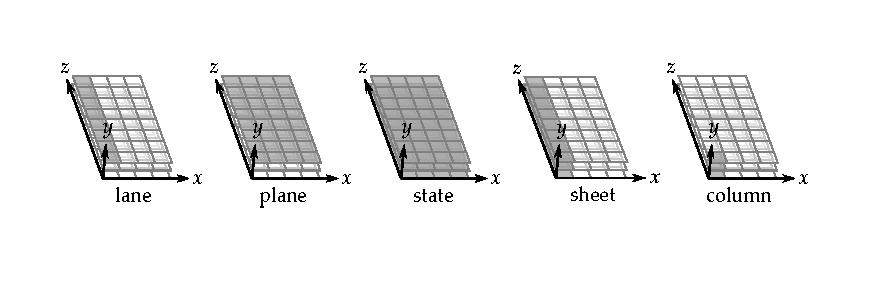
\includegraphics[width=1\textwidth]{figures/xoodooTerminology}
	\caption{Grafické znázornenie terminológie v XOODOO}
	\label{xoodooterm}
\end{figure}

Roviny majú index $y$. $y=0$ zodpovedá spodnej rovine a vrchná rovina $y=2$. Bit je označený s indexom $z$ vrámci množiny pruhov. List ich označujeme pomocou indexu $x$. Takže pozícia pruhu v stave je definovaná pomocou dvoch súradníc $(x,y)$. Konkrétny bit je možné v stave následne reprezentovať pomocou trojice súradníc $(x,y,z)$. Pri učení stĺpca sú potrebné 2 súradnice $(x,z)$. Pred spustením samotného algoritmu musí používateľ vykonať mapovanie 384-bitovej správy voči horizontálnym rovinám. Tento úkon sa realizuje pomocou matematickej formuly \ref{index}.

\begin{equation}\label{index}
	i=z+32(x+4y)
\end{equation}

Rundová funkcia pozostáva z 5 krokov:
\begin{enumerate}
	\item a	mixing layer $\theta$, 
	\item a plane shifting $\rho_{west}$, 
	\item the addition of round constants $\iota$,
	\item a non-linear layer $\chi$,
	\item an another plane shifting $\rho_{east}$.
\end{enumerate}
Celý algoritmus je znázornený pomocou schémy \ref{xoodooalgo}, ktorá je prebratá z \cite{xcb}. 

  \begin{figure}[!h]
  	\centering
  	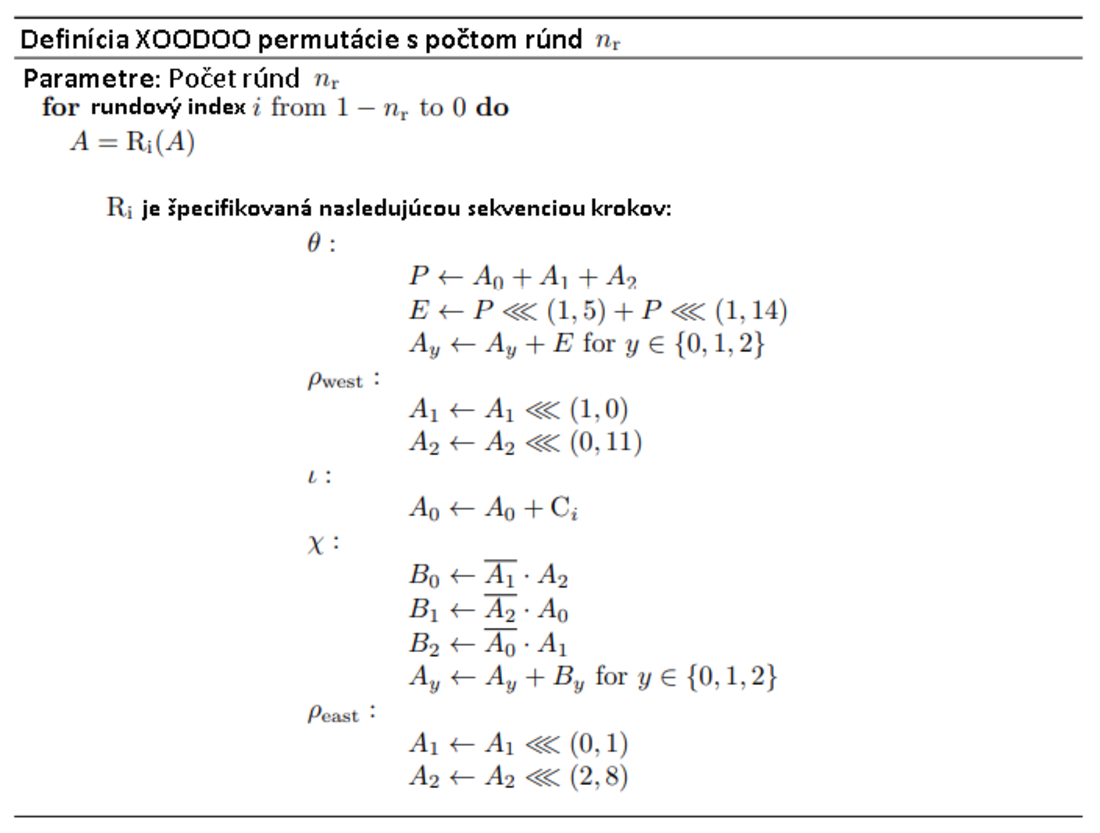
\includegraphics[width=1.1\textwidth]{figures/xoodooalgo}
  	\caption{}
  	\label{xoodooalgo}
  \end{figure}

\subsection{Xoodyak} 
Xoodyak možno považovať za všestranný kryptografický nástroj. Je vhodný pre väčšinu operácií využívajúcich symetrický kľúč. Napríklad generovanie pseudonáhodných bitov, autentizáciu, šifrovanie a mnohé iné. Tím Keccak použil pri návrhu duplexnú konštrukciu. Konkrétne variant s plným stavom a využitím kľúča. Tento dizajn označujeme ako \acrfull{fskd}. Viac o tejto konštrukcii si čitateľ môže prečítať v \cite{duplex}.
Operačný režim, v ktorom Xoodyak pracuje sa nazýva Cyklista -- z ang. \textit{Cyclist}. Tento názov získal ako opozitum k pomenovaniu režimu Motorista, ktorý je možné nájsť v Keyak schéme \cite{keyak}. Narozdiel od uvedeného balíka Keyak, nie je Xoodyak limitovaný len na autentizované šifrovanie. Je jednoduchší hlavne kvôli tomu že neobsahuje paralelné varianty.

\subsubsection{Režim Cyklista}\label{cyklista}
Režim Cyklista funguje na princípe kryptografických permutácií $f$, teda zmeny usporiadania bitov za pomoci tajného kľúča a matematických operácií. Parametrami sú veľkosti blokov $R_{hash}$, $R_{kin}$, $R_{kout}$ a veľkosť račety, resp. západky\footnote{z ang. \textit{the ratchet size}} \cite{ratchet} $\ell_{ratchet}$. Uvedený pojem sa v kryptografii používa vo forme obrazného pomenovania. Cieľom je poukázať na jednoduchý pohyb vpred, ale s ťažkým, resp. zložitejším pohybom naspäť. Dôležité je, že uvedený scenár je vyvolaný zámerným dizajnom. Šírka permutácie $b'$ je definovaná pomocou matematickej formuly \ref{index2}. Všetky uvedené parametre sú v bajtoch. Pre označenie prázdneho slova budeme používať $\epsilon$.
\begin{equation}\label{index2}
	max(R_{hash}, R_{kin}, R_{kout}) + 2 \leq b'
\end{equation} 

Cyklista operuje v dvoch režimoch -- \textbf{hašovací a kľúčový}\footnote{z ang. \textit{hash and keyed mode}.}. 
Inicializácia prebieha pomocou príkazu \lstinline|CYCLIST(K,id,counter)|. Ak sa parameter $K$ rovná prázdnemu slovu $\epsilon$, tak potom nastane spustenie v hašovacom režime. Aktuálne nie je do implementácie zakomponovaná možnosť zmeny režimu po inicializácií. Vývojári však túto vlastnosť nevylúčili pre prípadné aktualizácie balíka.  


Dostupné funkcie závisia od režimu, v ktorom sa  Cyklista spúšťa. Medzi ne patria \lstinline|ABSORB()| a \lstinline|SQUEEZE()|. Možno ich volať v oboch režimoch, zatiaľ čo funkcie \lstinline|ENCRYPT()|, \lstinline|DECRYPT()|, \lstinline|SQUEEZEKEY()| a \lstinline|RATCHET()| sú dostupné len pre kľúčový režim. Účel každej funkcie je nasledujúci:
\begin{itemize}
	\item \lstinline|ABSORB(X)| absorbuje vstupný reťazec X,
	\item C $\gets$ \lstinline|ENCRYPT(P)| zašifruje P do C a absorbuje P,
	\item P $\gets$ \lstinline|DECRYPT(C)| dešifruje C do P a absorbuje P,
	\item Y $\gets$	\lstinline|SQUEEZE($\ell$)|  vytvára $\ell$-bajtový výstup, ktorý závisí od doteraz absorbovaných dát,
	\item Y $\gets$	\lstinline|SQUEEZEKEY($\ell$)| funguje ako \lstinline|SQUEEZE($\ell$)|, ale používa sa za účelom generovania odvodeného kľúča, 		\\ell nefunguje v listings pckg
	\item \lstinline|RATCHET()| transformuje stav na nevratný tak, aby sa zabezpečila dopredná bezpečnosť\footnote{z ang. \textit{Forward secrecy}} \cite{fsec}. 
\end{itemize}

Stav bude závisieť od postupnosti volaní funkcií a od jeho vstupných reťazcov. Presnejšie povedané, zámerom je, že akýkoľvek výstup závisí od postupnosti všetkých vstupných reťazcov a volaní, tak že akékoľvek dva nasledujúce výstupné reťazce budú výstupom rôznych domén. Napríklad volanie \lstinline|ABSORB(X)| znamená, že výstup bude závisieť od reťazca $X$. Na druhej strane \lstinline|ABSORB()| vo funkcii \lstinline|ENCRYPT(P)| vytvorí výstup závislý aj od $P$ z funkcie šifrovania. Okrem uvedených závislostí ovplyvňujú výstup aj iné dizajnové riešenia. Príkladom je minimalizácia pamäťovej stopy. Vo výsledku teda výstup závisí od počtu predchádzajúcich volaní funkcie \lstinline|SQUEEZE()| a predtým spracovaných textov pomocou funkcií \lstinline|ENCRYPT()| a \lstinline|DECRYPT()|. Viac informácií o režime je dostupných v kapitole 7.2, publikácie \cite{xcb}. 

\subsubsection{Definícia a bezpečnosť}
Xoodyak je definovaný pomocou operatívneho režimu Cyklista nasledovne:
\begin{equation}
	CYCLIST[f,R_{hash},R_{kin},R_{kout},\ell_{ratchet}]
\end{equation} 
Kde jednotlivé parametre majú veľkosti:
\begin{enumerate}
	\item $f$ -- permutácia XOODOO so šírkou 48 bajtov (384 bitov),
	\item $R_{hash}$ -- 16 bajtov,
	\item $R_{kin}$ -- 44 bajtov,
	\item $R_{kout}$ -- 24 bajtov,
	\item $\ell_{ratchet}$ -- 16 bajtov.  
\end{enumerate}
Takto definované parametre algoritmu dokážu poskytnúť 128-bitovú bezpečnosť v oboch režimoch Cyklistu. Samozrejmosťou je, že v prípade kľúčového režimu, musí byť veľkosť kľúča rovná alebo väčšia ako 128 bitov. Viac informácií o kryptografickej bezpečnosti algoritmov je možné nájsť v \cite{sec}.

Viac informácií o bezpečnosti Xoodyak-a je možné nájsť v \cite{xcb, 7.3}, odkiaľ boli informácie čerpané.

\subsection{Možnosti použitia Xoodyak algoritmu}
Obsahom tejto podkapitoly sú uvedené postupy ako a za akých okolností je daný balík možné použiť. 
\subsubsection{Použitie hašovacieho režimu}
Xoodyak sa dá aplikovať ako hašovacia funkcia.
\subsubsection{Použitie kľúčového režimu}
\section{Kryptografický algoritmus Gimli} 
\section{Kryptografický algoritmus Simpira384} 

% !TEX root = ../thesis.tex
\chapter{Konfigurácia prostredia, metodika testovania a merania}
\section{Prostredie virtuálnych strojov pomocou VirtualBox}\label{merania}
Pri testovaní funkcionality VPN sme použili virtualizačný nástroj (daľej \acrshort{vm}) Virtual Box (ďalej \acrshort{vb}), spoločnosti Oracle, vo verzii 6.1.38. \acrshort{vb} je voľne dostupný. Inštalácia je jednoduchá a rýchla. Viac informácii o nástroji je možné dohľadať v \cite{vbox}.

Pre použitie je potrebné aby mal používateľ k dispozícií obraz operačného systému (ďalej \acrshort{os}). Tie nie je problém získať ani pre \acrshort{os} Windows a podobne, avšak pri našej práci sme zvolili využitie voľno dostupného  \acrshort{os} -- \textbf{Linux Ubuntu} vo verziách 22.04.3(\acrshort{lts}\footnote{z ang. \acrlong{lts}})-- OSC a následne vytvorili klon -- OSS. Pri opise práce použijeme označenia OSS pre VPN server a OSC pre klienta.

Pri jednoduchej inštalácií \acrshort{vm} sme použili konfiguráciu s  2048 MB RAM a 2 jadrami. (Minimálna inštalácia). V prípade potreby dávame do popredia návod na prípravu Windows \acrshort{os} v \acrshort{vm} -- \cite{vmkonfig}, avšak postup je triviálny. Po inštalácii sme OS aktualizovali pomocou príkazov:
\begin{lstlisting}[language=bash]
	sudo apt-get update
	sudo apt-get upgrade
\end{lstlisting}
Následne sme doinštalovali potrebné súčasti k \acrshort{vm} \acrshort{os} vo verzii ako je \acrshort{vb}, teda 6.1.30. Dôvodom bolo zväčšenie rozlíšenia a využívanie možnosti zdieľaného priečinka s \acrshort{os}, na ktorom daný \acrshort{vb} beží. Za účelom správneho fungovania priečinka bolo nutné v termináli použiť príkaz:
\begin{lstlisting}[language=bash]
	sudo usermod -aG vboxsf $(whoami)
\end{lstlisting}
a následne reštartovať \acrshort{os}.

Posledné úpravy prostredia sú spojené s jazykom C a balíčkom Make. Inštalácia je opäť jednoduchá. Použili sme príkazy:
\begin{lstlisting}[language=bash]
	sudo apt install gcc
	sudo apt install make
\end{lstlisting}
Uvedené úpravy boli vykonané na oboch \acrshort{os}.

V prípade použitia \acrshort{os} Windows je postup inštalácie jazyka C a balička Make zložitejší. Používateľovi odporúčam použitie knižníc Winlibs\footnote{dostupne na \href{https://winlibs.com/}{https://winlibs.com/}}. Po stiahnutí balíčkov musí používateľ importovať uvedený balíček, resp. cestu k nemu, do premenných prostredia \acrshort{os} Windows. Jeden zo spôsobov je uvedený aj na Winlibs stránke. 

\subsection{Zmena sieťových adaptérov}
\acrshort{vb} ponúka rôzne možnosti nastavenia sieťových adaptérov. Aktuálne su dostupné tieto:
\begin{itemize}
	\item{Not attached}
	\item{Network Address Translation (ďalej NAT)}
	\item{NAT Network}
	\item{Bridge adapter}
	\item{Internal}
	\item{Host-Only}
	\item{Generic driver}
	\item{Cloud-Based} -- experimentálne
\end{itemize} 
 
Konektivita jednotlivých možností je znázornená pomocou obrázku \ref{vbmode}. Viac informácií o jednotlivých režimoch je dostupných na \cite{vboracle}.

\begin{figure}
	\centering
	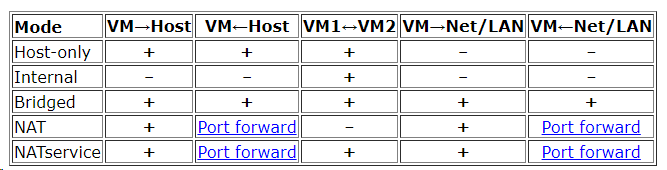
\includegraphics[width=.9\textwidth]{figures/vbmodes}
	\caption{Konektivita jednotlivých sieťových adaptérov}
	\label{vbmode}
\end{figure}
Vzhľadom k našim potrebám, teda obojsmerná komunikácia medzi 2 VM, sú pre nás relevantné režimy bridge a NAT network. Ako si môžeme všimnúť, NAT vyžaduje dodatočnú konfiguráciu portov v prípadoch kedy chceme aby nastala komunikácia medzi dvoma VM. Z tohto dôvodu je pre čo najjednoduchší prístup zvoliť práve režim bridge. Ten priradí VM vlastnú IP adresu, pomocou, ktorej stroj komunikuje. 

Viac o jednotlivých režimov je taktiež možné nájsť v \cite{vbguide}. Autor sa venuje postupu konfigurácie jednotlivých režimov spoločne s ich opisom.

\section{Nástroje použité v obrazoch a v práci}
  \subsubsection{Winlibs balík}
  \subsubsection{Visual studio Code}
  \subsubsection{GCC prekladač a balík Make}
  \subsubsection{Tunelovacie rozhranie Wintun}
  \subsubsection{Zdrojový kód na meranie počtu cyklov a času} 
  \subsubsection{Umelá inteligencia založená na GPT3/4} 
   
\chapter{Implementacia jednoduchej VPN siete}
Za účelom demonštrácie jednoduchej VPN siete sme zvolili voľne dostupnú implementáciu v jazyku C. V tejto kapitole postupne rozoberieme funkcionalitu a správanie vzniknutej VPN siete.
\section{Dead Simple VPN}\label{dsvpn}
Dead Simple VPN je voľne dostupný\footnote{\href{https://github.com/jedisct1/dsvpn}{https://github.com/jedisct1/dsvpn}} program, napísaný v jazyku C. Určený je pre operačný systém Linux. Autorom je Frank Denis. DSVPN rieši najbežnejší prípad použitia VPN, teda pripojenie klienta k VPN serveru cez nezabezpečenú sieť. Následne sa klient dostane na internet prostredníctvom servera. Uvedenú skutočnosť je možne vidieť na schéme \ref{vpnsimple}.
\begin{figure}
	\centering
	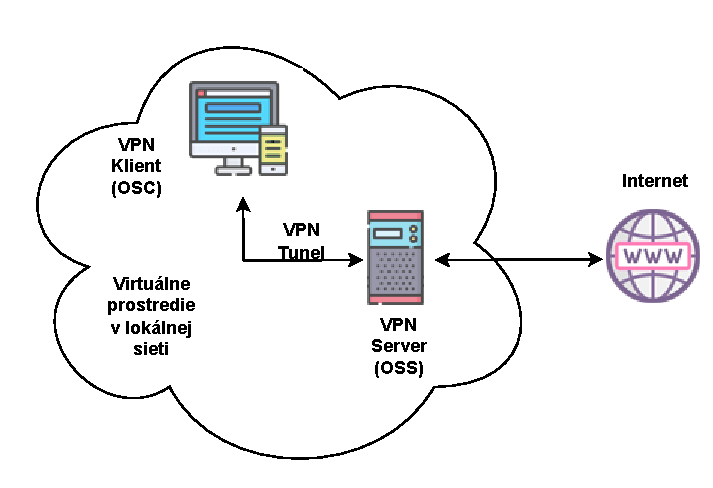
\includegraphics[width=0.9\textwidth]{figures/vpnsimple}
	\caption{Schéma jednoduchej VPN}
	\label{vpnsimple}
\end{figure}

DSVPN používa protokol riadenia prenosu -- \acrshort{tcp} \cite{tcp}. Medzi ďalšie pozitíva patrí:
\begin{itemize}
	\item{Používa iba modernú kryptografiu s formálne overenými implementáciami.}
	\item{Malá a konštantná pamäťová stopa. Nevykonáva žiadne dynamické alokovanie pamäte (z ang. \textit{heap memory}).}
	\item{Malý (~25 KB) a čitateľný kód. Žiadne vonkajšie závislosti (z ang. \textit{Dependencies}).}
	\item{Funguje po preklade GCC prekladačom. Bez dlhej dokumentácia, žiaden konfiguračný súbor, dodatočná konfigurácia. DSVPN je spustiteľná jednoriadkovým príkazom na serveri, obdobne na klientovi. Bez potreby konfigurácie brány firewall a pravidiel smerovania.}
	\item{Funguje na Linuxe (kernel $\geq$ 3.17), macOS a OpenBSD, DragonFly BSD, FreeBSD a NetBSD v klientskych a point-to-point režimoch. Pridanie podpory pre iné operačné systémy je triviálne.}
	\item{Nedochádza k úniku IP medzi pripojeniami, ak sa sieť nezmení. Blokuje IPv6 na klientovi, aby sa zabránilo úniku IPv6 adries.}
\end{itemize} 

V uvedenej VPN autor zakomponoval aj možnosť pokročilejších nastavení. Celkový súhrn vstupných parametrov pri štarte programu je takýto:
\begin{lstlisting}[language=bash]
	./dsvpn   server
	<key file>
	<vpn server ip or name>|"auto"
	<vpn server port>|"auto"
	<tun interface>|"auto"
	<local tunnel ip>|"auto"
	<remote tunnel ip>"auto"
	<external ip>|"auto"

	./dsvpn   client
	<key file>
	<vpn server ip or name>
	<vpn server port>|"auto"
	<tun interface>|"auto"
	<local tunnel ip>|"auto"
	<remote tunnel ip>|"auto"
	<gateway ip>|"auto"
	\end{lstlisting} 
Väčšina parametrov je v zdrojovom kóde prednastavených na automatické hodnoty. Príkladom je port 443, vytvorenie rozhrania tun0, prevzatie externej IP adresy zo siete a ďalšie. Používateľ teda môže spúštať DSVPN pomocou príkazu s najmenej 2 parametrami v prípade servera a tromi pre prípad klienta. Dôvodom je, že klient potrebuje mať určenú IP adresu servera, na ktorý sa má pripojiť (3.parameter). Druhý parameter v poradí je už spomenutá cesta k zdieľanému 256-bitovému kľúču.   

\section{Kryptografia použitá v DSVPN}
DSVPN používa v svojej implementácií malú sebestačnú kryptografickú knižnicu -- \textit{Charm}\footnote{\url{https://github.com/jedisct1/charm}}. Jej autorom je tvorca DSVPN. Implementácia umožňuje autentizované šifrovanie (z ang.\textit{authenticated encryption}) a hašovanie kľúčov (z ang. \textit{keyed hashing}). Správnosť implementácie algoritmu v knižnici programátor overil pomocou nástroja \textbf{Cryptol}\footnote{\url{https://cryptol.net/index.html}}. Uvedený nástroj slúži na zápis algoritmu do matematickej špecifikácií. Tým poskytne možnosť jednoduchšej a hlavne korektnej implementácie zvoleného kryptografického algoritmu. Zároveň je možné program využiť aj na verifikáciu vytvoreného riešenia. Obdobne sú v repozitári knižnice ponechané overovacie skripty pre jednoduché spustenie. 

Kryptografický algoritmus použitý v DSVPN je Xoodoo permutácia v duplex móde, pričom môže byť jednoducho nahradená napríklad Gimli-im\footnote{\url{https://github.com/jedisct1/gimli}} \cite{gimli} alebo Simpira384\footnote{\url{https://github.com/jedisct1/simpira384}} \cite{simpira}. Pri zmene musí používateľ zasiahnuť do zdrojového kódu v súbore \textbf{charm.c}, ktorého obsahom sú kryptografické primitíva.     
\section{Experimentálne overenie VPN}
DSVPN sme prakticky overili pomocou dvojice virtuálnych strojov OSS a OSC, ktorých opis je obsahom \ref{merania}. Na zariadení OSS sme pomocou balička make a GCC prekladača vykonali inštaláciu DSVPN. Obdobný postup je aplikovaný aj vo VM OSC. Na OSS spúšťame VPN Server, ktorý nám poskytne IP adresu, prostredníctvom ktorej budeme komunikovať s vonkajším svetom. Na spustenie a vytvorenie spojenie vykonáme nasledujúce úkony:
\begin{enumerate}
	\item Vygenerovanie zdieľaného kľúča:\begin{lstlisting}[language=bash]
		dd if=/dev/urandom of=vpn.key count=1 bs=32
	\end{lstlisting} 
-- zdieľaný kľúč, ktorý sme vygenerovali, sa nám uložil do súboru \textit{vpn.key}. Jeho veľkosť je 32 bajtov, teda 256 bitov. Kľúč je potrebné vložiť do priečinka s programom \textit{dsvpn} v oboch zariadeniach -- OSS aj OSC alebo zadať cestu ako parameter, kde sa kľúč nachádza.
	\item OSS zariadenie: \begin{lstlisting}[language=bash] 
	sudo ./dsvpn server vpn.key auto 
	2340 auto 10.8.0.254 10.8.0.2
	\end{lstlisting} 
-- tento príkaz zabezpečí spustenie VPN servera na prostredí OSS s IP adresou. Príkaz \lstinline|sudo| nám spustí program s administrátorskými právami. Piaty parameter nastavuje IP adresu servera. V našom prípade \lstinline|auto|, použije aktuálne používanú IP na komunikáciu s vonkajším prostredím. Príkazom ďalej definujeme portové číslo 2340, ktoré sa použije pri nastolení TCP spojenie medzi klientom a serverom. Poslednou konfiguráciou je priradenie mena a IP adresy tunelov, ktoré bude využívať naše zariaadenie -- 10.8.0.254 a druhý koniec tunela -- 10.8.0.2. Používateľ má ešte možnosť nastaviť tzv. External IP. Tú by sme využili ak by sme spúšťali DSVPN na routri poskytovateľa internetu. Obdobne na klientovi vieme nastaviť gateway IP, ktorá slúži na presmerovanie komunikácie k serveru. Po spustení príkazu si vieme overiť našu konfiguráciu\footnote{Pomocou \lstinline|ip address show tun0| overíme IPv4 adresu VPN tunela.}. 
	\item OSC zariadenie: \begin{lstlisting}[language=bash] 
	sudo ./dsvpn client vpn.key 192.168.88.62 
	2340 auto 10.8.0.2 10.8.0.254
	\end{lstlisting} 
-- uvedený príkaz zabezpečí, že sa pripojíme na VPN Server, ktorý ma ip adresu \textit{192.168.88.62} s portom 2340. Následne vzniká TCP spojenie. Dôležité je si všimnúť poradie adries tunelov. Je opačné ako v prípade servera. 
	\item V prípade úspešnej konektivity sa operácia podarila a pre okolitý svet sme viditelný pomocou IP adresy, ktorú sme zvolili. 
\end{enumerate}

Na overenie správnosti funkcionality nám postačí jednoduchý sieťový príkaz \lstinline|traceroute|. Napríklad \lstinline|traceroute google.sk|\footnote{vo Windows CMD prostredí: \lstinline|tracert google.sk|}. Prvá z uvedených adries je práve tá, ktorú dané zariadenie používa. 

V našom prípade bolo nutné použiť lokálne adresy vzhľadom na to, že obe VM bežia na jednom hosťovskom počítači. Obidva zariadenia sú tým pádom pripojené k jednému internetovému poskytovateľovi, čo má za následok takmer rovnaké smerovanie k vzdialenej doméne. 

Proces zistenia IP adresy VPN servera, po spustení, a overenie funkčnosti je následne znázornené pomocou \ref{ipu21},\ref{ipu20}, \ref{vpntru20}.
V  \ref{ipu21} sme žltou farbou znázornili IP adresu, na ktorej je VPN server dostupný. Oranžová farba znázorňuje IP adresy tunelu medzi serverom a klientom v tomto poradí. Následne v \ref{ipu20} môžeme vidieť to isté pre klienta.
  \begin{figure}
  	\centering
  	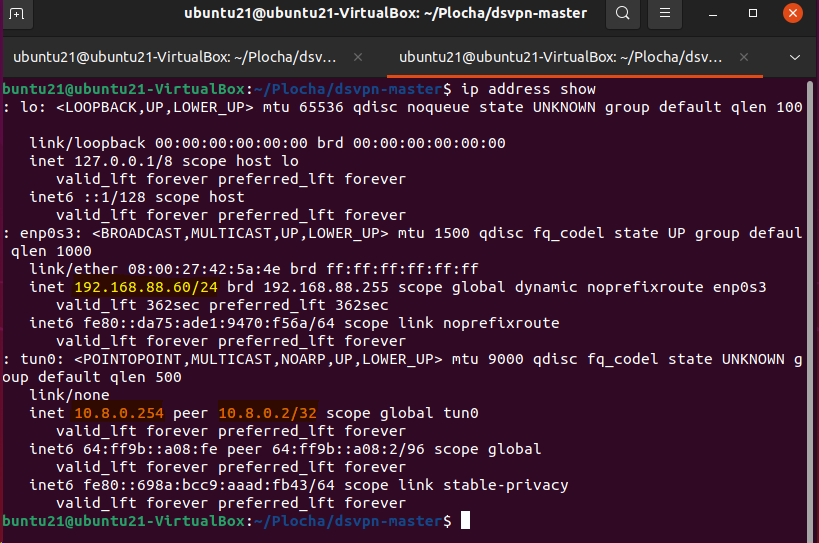
\includegraphics[width=0.9\textwidth]{figures/ipu21}
  	\caption{Zistenie IP adries VPN Servera na VM OSS}
  	\label{ipu21}
  \end{figure}
  

\begin{figure}
	\centering
	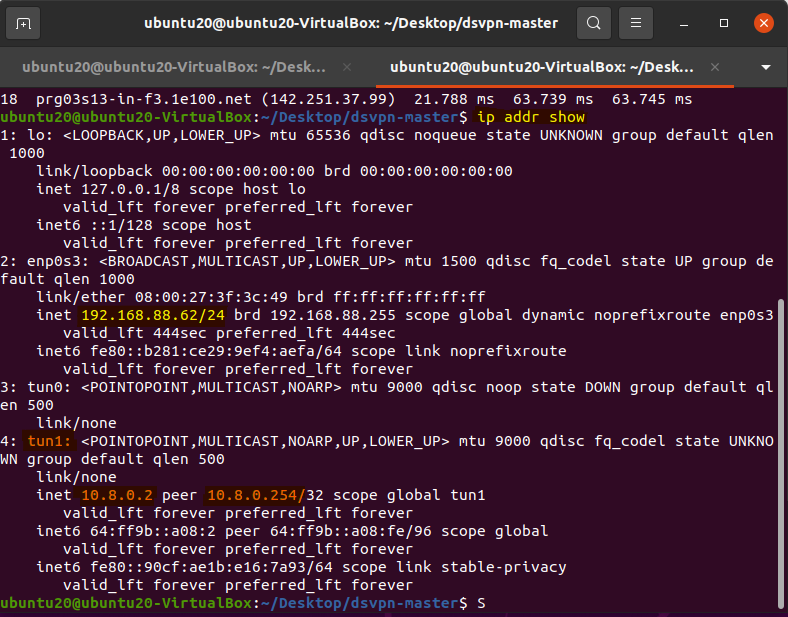
\includegraphics[width=0.9\textwidth]{figures/ipu20}
	\caption{Zistenie IP adries VPN Klienta na VM OSC}
	\label{ipu20}
\end{figure}
Nakoniec, v \ref{vpntru20} môžeme vidieť ako klient pri internetovej komunikácií používa namiesto svojej vlastnej, adresu poskytnutú VPN Serverom na zariadení OSS -- žltou zvýraznená IP. Červenou je zaškrnutá farba poskytovateľa internetu. 

\begin{figure}
	\centering
	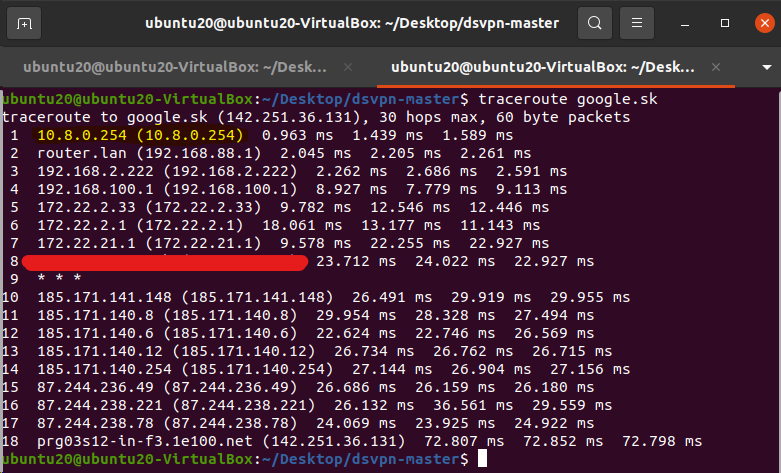
\includegraphics[width=0.9\textwidth]{figures/vpntru20}
	\caption{Overenie funkcionality DSVPN pomocou traceroute}
	\label{vpntru20}
\end{figure}
\section{Princíp fungovania programu}
DSVPN vytvára VPN sieť medzi VPN klientom a VPN serverom. Na obidvoch zariadeniach je potrebné spustiť program pomocou korešpondujúcich príkazov. 

Princíp vysvetlíme na praktickom príklade. Klienta umiestnime na lokálnu sieť bez prístupu na internet. Následne vymažeme všetky smerovacie pravidlá v zariadeni. Klient po tomto kroku nedokáže komunikovať so žiadným zariadením nakoľko nemá žiadne prednastavené pravidlá kam by smeroval internetovú komunikáciu. V uvedenej lokálnej sieti bude prítomný taktiež VPN server, ktorý ako jediný dokáže komunikovať s okolitým svetom. Po spustení DSVPN na obidvoch zariadeniach, dochádza k spojeniu. Jedná sa o TCP spojenie vytvorené soketmi. Úlohou soketového TCP spojenia je preposielanie už zašifrovaných dát v novom L3 pakete.  Následne DSVPN overuje stav soketov a tunelovacieho rozhrania. Ak je tun rozhranie pripravené na čítanie (obsahuje pakety), tak dochádza k ich spracovaniu (šifrovaniu) a preposlaní cez soket. Po prijatí sa dáta dešifrujú a smerujú na základe dát z L3 IP hlavičky. 

Toto je celý princíp zabezpečenej komunikácie medzi Klientom a Serverom vo VPN sieti na L3 vrstve. Aby sme docielili plnohodnotnú funkcionalitu VPN, tak potrebujeme do tohto riešenia zakomponovať smerovanie. Tým, že dáta smerujeme von z tejto siete, tak je ešte potrebné upraviť niektoré systémové smerovacie pravidla.      

Okrem načrtnutého príkladu s prístupom na internet, dokáže klient takto získať konektivitu k jemu nedostupným segmentom siete. Samozrejme za predpokladu, že sú dostupné pre server. Ako príklad môže byť diskové úložisko. Prípadne prístup na internetové domény. V angličtine sa takýto termín označuje ako \textit{remote access}, teda vzdialený prístup. Je to tiež veľmi obľúbený a používaný typ VPN siete. 

Funkcionalita DSVPN je znázornená pomocou schémy \ref{dsvpnarch}. V nej môžeme na ľavej strane vidieť čo sa deje s paketom pri požiadavke smerom od VPN klienta k VPN serveru. OS na základe požiadavky formoju L3 pakety. Po presmerovaní paketu na tunel DSVPN zašifruje tieto dáta. Následne ich zapíše na soket, ktorý tvorí so serverom TCP spojenie. Server tieto dáta spracuje a vykoná potrebné náležitosti. Po získaní odpovede zasa Server odpovedá klientovi rovnakým mechanizmom. Čitateľovi by som rád doplnil, že v schéme sme pre DSVPN vytvorili 2 bloky. \textbf{DSVPN IN} a \textbf{DSVPN OUT}. Funkcionalita je znázornená iba v spodnej časti schémy. Jedná sa však o identické bloky.
% TODO: \usepackage{graphicx} required
\begin{figure}[h!]
	\centering
	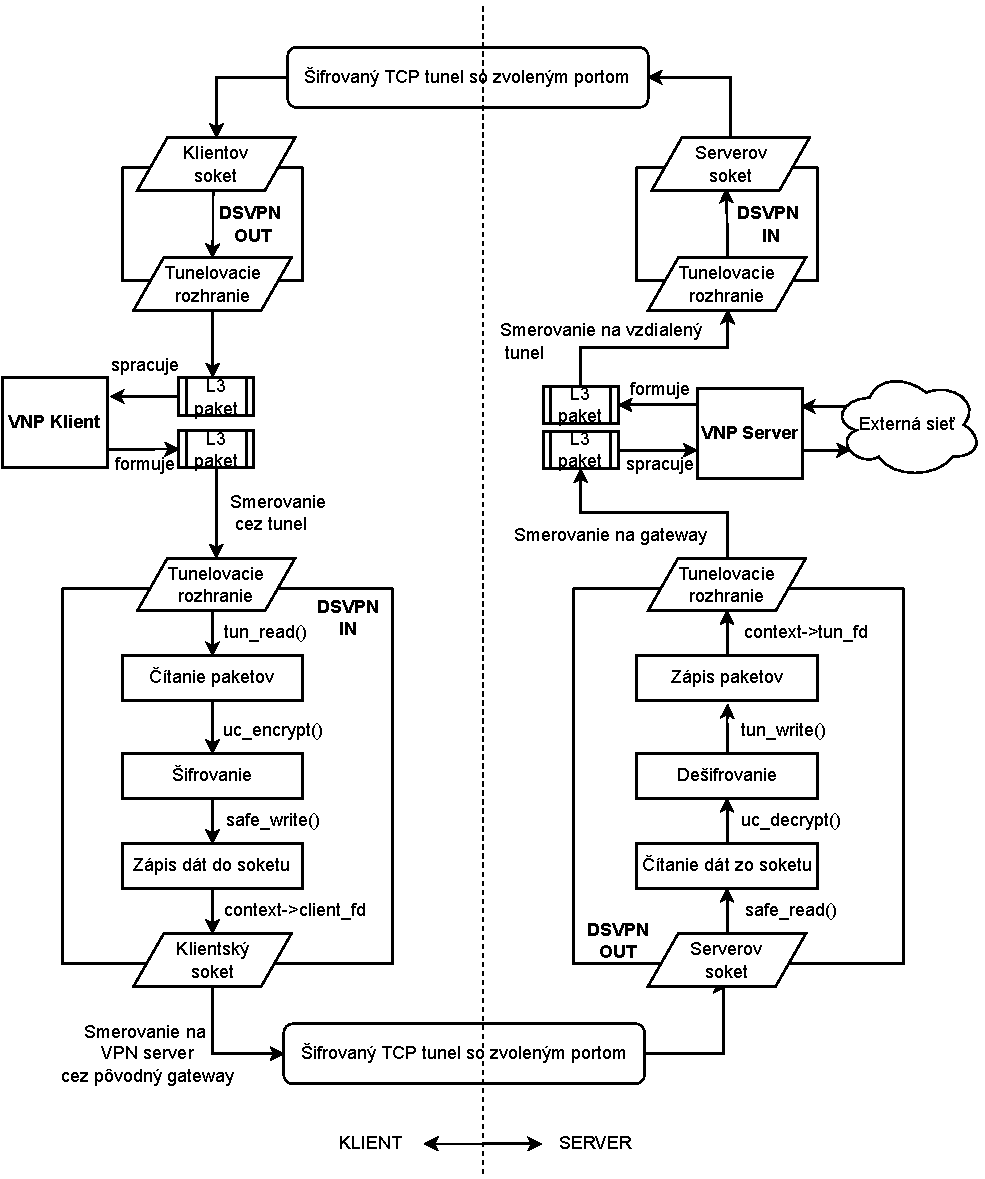
\includegraphics[width=1.1\textwidth]{figures/dsvpn.pdf}
	\caption{Ukážka prenosu paketu naprieč DSVPN}
	\label{dsvpnarch}
\end{figure}


 
\section{Analýza zdrojového kódu DSVPN}
Pri analýze sa zameriame výhradne na dôležité časti kódu DSVPN pre programovací jazyk C. Repozitár pozostáva z jedného make-file balíčka\cite{make}. 3 hlavičkových (.h) a k ním korešpondujúcimi zdrojovými kódmi (.c), s pomenovaním:
 \begin{enumerate}
 	\item \textbf{charm.h} -- kryptografická knižnica so 6 funkciami,
 	\item \textbf{os.h} -- funkcie čítania a zápisu paketov, vytvorenia, používania a zrušenia tunelovacieho rozhrania,
 	\item \textbf{vpn.h} -- deklarácia konštánt, endianity\cite{endianita} a niektorých závislostí OS.
 \end{enumerate}

V spomenutých hlavičkových súboroch sa nachádzajú deklarácie funkcií, ktoré VPN používa. Definície sú obsahom .c súborov, ako je v jazyku C zaužívaným zvykom. Obsahom tejto podkapitoly je analýza týchto kódov. 
 
\subsection{Súbor charm.h a charm.c}
Obsahom sú prevažne funkcie slúžiace pri behu kryptografického algoritmu XOODOO. Charm.h pozostáva z 6 funkcií. Ich implementácia nie je až tak rozsiahla. Zaberá celkovo 337 riadkov. Princípy použité v algoritme bolí opísané v kapitole 2.  
 
   \begin{minipage}{\linewidth} 	
  	\begin{lstlisting}[frame=single,
  		numbers=left,
  		caption={Obsah charm.h}\label{charm.h},
  		basicstyle=\ttfamily\small, keywordstyle=\color{black}\bfseries,]
void uc_state_init(uint32_t st[12], const unsigned char key[32], 
				  			 	 const unsigned char iv[16]);
void uc_encrypt(uint32_t st[12], unsigned char *msg, 
							  size_t msg_len, unsigned char tag[16]);	
int uc_decrypt(uint32_t st[12], unsigned char *msg, 
			   			   size_t msg_len,
			   			   const unsigned char *expected_tag, 
			   			   size_t expected_tag_len);
void uc_hash(uint32_t st[12], unsigned char h[32],
			 			 const unsigned char *msg, size_t len);
void uc_memzero(void *buf, size_t len);
void uc_randombytes_buf(void *buf, size_t len);
  		 	\end{lstlisting}
  	\end{minipage}\\
Z názvov funkcií je pomerne jasné čo sa v jednotlivých volaniach deje.   
 \subsection{Súbor os.h a os.c}
Obsahom su funkcie, ktorých úlohami sú čítanie alebo pridanie \acrshort{gw}, vytvorenie a nastavenie tunelu v danom OS. Následne je aplikovaná úprava firewall pravidiel, tak aby všetka komunikácia bola presmerovaná na VPN server. Úprava firewall pravidiel je závislá od role, pod ktorou je VPN spustená. Teda či sa jedná o server alebo klienta. 
Celkovo je obsahom 12 funkcií, ktoré riešia uvedené úlohy. Detail je možné vidiet v \ref{os.h}.
 
 \begin{minipage}{\linewidth} 	
	\begin{lstlisting}[frame=single,
		numbers=left,
		caption={Obsah ZK os.h}\label{os.h},
		basicstyle=\ttfamily\small, keywordstyle=\color{black}\bfseries,]
 ssize_t safe_read(const int fd, void *const buf_, size_t count, 
 						       const int timeout);
 ssize_t safe_write(const int fd, const void *const buf_, 
 							      size_t count,
 							      const int timeout);
 ssize_t safe_read_partial(const int fd, void *const buf_,
 							 					   const size_t max_count);
 ssize_t safe_write_partial(const int fd, void *const buf_, 
 							    		     	const size_t max_count);
 
 typedef struct Cmds {
 	const char *const *set;
 	const char *const *unset;
 } Cmds;
 
 Cmds firewall_rules_cmds(int is_server);
 int shell_cmd(const char *substs[][2], const char *args_str,
 			         int silent);
 const char *get_default_gw_ip(void);
 const char *get_default_ext_if_name(void);
 int tcp_opts(int fd);
 int tun_create(char if_name[IFNAMSIZ], const char *wanted_name);
 int tun_set_mtu(const char *if_name, int mtu);
 ssize_t tun_read(int fd, void *data, size_t size);
 ssize_t tun_write(int fd, const void *data, size_t size); 
\end{lstlisting}
\end{minipage}\\ 
Samozrejmosťou je implementácie čítania a zápisu dát z TUN tunelu, soketu a príkazového riadku. 
 \subsection{Súbor vpn.h a vpn.c}
 Hlavičkový súbor obsahuje prevažne definovanie niektorých parametrov potrebných na správnu funkcionalitu VPN, spoločne s korekciou pre niektoré OS. Viď. \ref{vpn.h}. Ostatné parametre, ktoré bolí opísané pre spustenie, su definované práve v tomto súbore (porty, IP adresy, MTU atď.).
 
 \begin{minipage}{\linewidth} 	
 	\begin{lstlisting}[frame=single,
 		numbers=left,
 		caption={Obsah ZK vpn.h}\label{vpn.h},
 		basicstyle=\ttfamily\small, keywordstyle=\color{black}\bfseries,]
 /*UNIX-like OS Dependent Libraries*/
 #include <sys/ioctl.h>
 #include <sys/socket.h>
 #include <sys/types.h>
 #include <sys/uio.h>
 #include <sys/wait.h>
 #include <net/if.h>
 #include <netinet/in.h>
 #include <netinet/tcp.h>
 /*End UNIX-like OS Dependent Libraries*/
 /*OS setup dependencies*/
 #ifdef __linux__
 #include <linux/if_tun.h>
 #endif
 
 #ifdef __APPLE__
 #include <net/if_utun.h>
 #include <sys/kern_control.h>
 #include <sys/sys_domain.h>
 #endif
 
 #ifdef __NetBSD__
 #define DEFAULT_MTU 1500
 #else
 #define DEFAULT_MTU 9000
 #endif
 /*End of OS setup dependencies*/ 
 	\end{lstlisting}
\end{minipage}\\

\subsubsection{Main() -- Beh programu}
Pred samotným opisom by som rád upozornil na jeden fakt. Autor DSVPN používa vo veľkej miere zápis pomocou tzv. ternárnych operátorov. Viac informácií o tejto problematike je možné nájsť v \cite{ternary}. V skratke, používa sa podmienený zápis hodnoty do premennej.

Vpn.c je hlavným zdrojovým kódom DSVPN. V jeho vnútri nájdeme hlavnú, štartovaciu, funkciu main. Zároveň má prilinkované aj vyššie uvedené knižnice. Ako prvé dochádza k inicializácií premennej štruktúry \lstinline|Context|\ref{context}. Štruktúra v sebe nesie všetky premenné, potrebné na správne fungovanie programu.

\begin{minipage}{\linewidth} 	
	\begin{lstlisting}[frame=single,
		numbers=left,
		caption={Štruktúra Context}\label{context},
		basicstyle=\ttfamily\small, keywordstyle=\color{black}\bfseries,]
typedef struct Context_ {
	const char *  wanted_if_name;
	const char *  local_tun_ip;
	const char *  remote_tun_ip;
	const char *  local_tun_ip6;
	const char *  remote_tun_ip6;
	const char *  server_ip_or_name;
	const char *  server_port;
	const char *  ext_if_name;
	const char *  wanted_ext_gw_ip;
	char          client_ip[NI_MAXHOST];
	char          ext_gw_ip[64];
	char          server_ip[64];
	char          if_name[IFNAMSIZ];
	int           is_server;
	int           tun_fd;
	int           client_fd;
	int           listen_fd;
	int           congestion;
	int           firewall_rules_set;
	Buf           client_buf;
	struct pollfd fds[3];
	uint32_t      uc_kx_st[12];
	uint32_t      uc_st[2][12];
} Context;   
 	\end{lstlisting}
\end{minipage}\\ 

 Následne dochádza k načítaniu vopred zdieľaného kľúča pomocou pomocnej funkcie 
\\
 \lstinline|load_key_file()|\ref{load}. Úlohou je prečítanie kľúča, pričom sa používa funkcia z os.c -- \lstinline|safe_read()|. Realizuje sa znakové spočítanie, v ktorom je zakomponovaná funkcia  \lstinline|poll()| \cite{poll}. Dôvodom je, že \lstinline|safe_read()| sa používa aj pri čítaní zo soketu a tunelu. V linuxe je čítanie z týchto typov rovnaké. Tato časť kódu je však podmienená špecifickou chybou, ktorú je možné dostať len pri čítaní soketu, respektíve tunelu.  
 V prípade, ak sa prečítalo 32 bajtov, \lstinline|safe_read()| vracia 0. Následne sa inicializuje stav v XOODOO.
 
 \begin{minipage}{\linewidth} 	
 	\begin{lstlisting}[frame=single,
 		numbers=left,
 		caption={Načítanie zdieľaného kľúča}\label{load},
 		basicstyle=\ttfamily\small, keywordstyle=\color{black}\bfseries,]
 static int load_key_file(Context *context, const char *file)
 {
 	unsigned char key[32];
 	int           fd;
 	
 	if ((fd = open(file, O_RDONLY)) == -1) {
 		return -1;
 	}
 	if (safe_read(fd, key, sizeof key, -1) != sizeof key) {
 		(void) close(fd);
 		return -1;
 	}
 	uc_state_init(context->uc_kx_st, key, 
 							 (const unsigned char *) "VPN Key Exchange");
 	uc_memzero(key, sizeof key);
 	
 	return close(fd);
 }
  	\end{lstlisting}
\end{minipage}\\ 
Ako môžeme vidieť v implementácii sú bežne použité smerníky. Vo výsledku tak dokážeme preniesť zmenu hodnôt na viaceré premenné.
 
V prípade, ak používateľ pri štarte nezmenil parameter pre IP adresu sieťovej brány\footnote{z ang. \textit{GateWay}} (ďalej \acrshort{gw}), tak sa používa pôvodná. Tá sa získa pomocou funkcie \\\lstinline|get_default_gw_ip()|, ktorá je deklarovaná v \ref{os.h}. Prostredníctvom shell príkazu \lstinline|ip route| a \lstinline|read_from_shell_command()| funkcie, dochádza k extrakcii informácií priamo z príkazového riadka. Tento krok je teda závislý od \acrshort{os}, v ktorom používateľ pracuje. Nasleduje overenie návratových hodnôt z funkcií iba v prípade ak je DSVPN spustené ako Klient.
 
Program v prípade servera pokračuje s \lstinline|get_default_ext_if_name()|. Obdobne ako v predchádzajúcom odstavci je realizácia funkcionality, vykonaná pomocou terminálu. Podstata spočíva v zistení mena tunelovacieho rozhrania.
 
Po nastavení parametrov sa dostávame k vytvoreniu tunelovacieho rozhrania. V tomto kroku autor používa funckiu \lstinline|tun_create|. Úloha je vysoko závislá od OS. Dôsledkom toho je možné vidieť vetvenie funkcionality vzhľadom k bežiacemu OS. DSVPN poskytuje kompatibilitu pre 6 OS, medzi, ktoré patrí Linux, FreeBSD, NetBSD, OpenBSD, MacOS, DragonFly. Následne na základe systému dochádza k vytváraniu tunelu s prednastaveným, resp. zvoleným menom. Program ďalej nastaví maximálnu veľkosť prepravovaného paketu\footnote{z ang. \textit{Maximum Transmission Unit}} (ďalej \acrshort{mtu}) na 1500/9000 bajtov. 
 
Po príprave tunelu dochádza k overeniu dostupnosti VPN servera. Tento krok vykonáva funkcia \lstinline|resolve_ip|. Tá ma v sebe vnorené 2 funkcie, ktoré su menným ekvivalentom aj vo Windows knižniciach. Jedná sa o funkcie \lstinline|getaddrinfo| a \lstinline|getnameinfo|.  
 
Posledným krokom súvisiacim s konfiguráciou prostredia je vytvorenie pravidla pre branu FireWall (ďalej \acrshort{fw}). Tento úkon realizuje \lstinline|firewall_rules()|. Tento proces je opäť systémovo závislý. Jeho realizácia je vykonaná pomocou globálne definovanej funkcie \lstinline|Cmds firewall_rules_cmds()|. Tá obsahuje súbor prednastavených príkazov. Ich úlohou je presmerovanie celej premávky cez vzniknutý tunel.
 
Posledným úkonom je samotný beh VPN. Ten spúšťa funkcia \lstinline|doit()|. Doterajší beh programu je jednoducho znázornený pomocou flow diagramu \ref{fc1}.
 
\begin{figure}
	\centering
	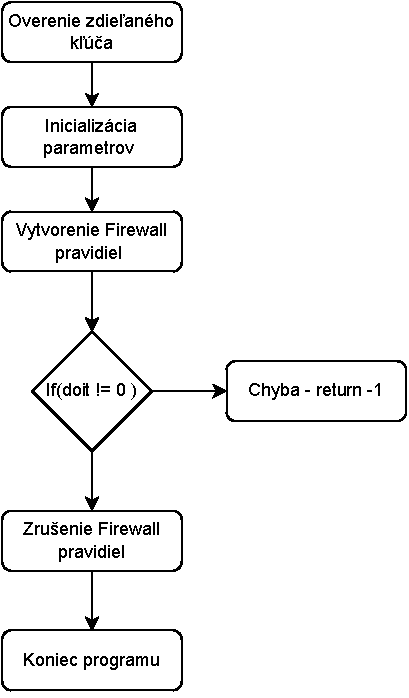
\includegraphics[width=0.5\textwidth]{figures/fc1}
	\caption{Beh DSVPN}
	\label{fc1}
\end{figure}

Od tohto momentu sa presúvame k postupnému vnáraniu do procesu spojenia a spracovania dát. Hlavnou úlohou funkcie \lstinline|doit()| je nadviazanie soketového TCP spojenia medzi klientom a serverom. Vo vnútri \lstinline|doit()| preto dochádza k vetveniu programu. V prípade, že je DSVPN spustená ako server spustí sa funkcia \lstinline|tcp_listener()|. V opačnom prípade \lstinline|client_reconnect()|. Listener vytvára socket a následne pomocou systemovej funkcie \lstinline|bind()| sa napojí na zvolený port. Potom čaká na spojenie od klienta pomocou funkcie \lstinline|listen()|. Smerník na socket je uložený do smerníka na štruktúru Context.
Klient používa vetvu s \lstinline|Client_reconnect()|. V nej sa snaží opakovane nadviazať spojenie so serverom. Za týmto účelom \lstinline|client_connect()|. Pred týmto úkonom samozrejme dochádza k overeniu či už nedošlo k nadviazaniu spojenia. O to sa stará \lstinline|client_disconnect()|, ktorý ruší aktívne spojenie.

\lstinline|Client_connect()| slúži na pripojenie klienta k serveru. Vykonáva aj úpravu pravidiel v \acrshort{fw}. Následne sa pokúša o nadviazania spojenia pomocou funkcie  \lstinline|tcp_client()|. Po tejto sérií úloh sa vraciame opäť do \lstinline|doit()|. V cykle \lstinline|while| sa vykonávaná funkcia \lstinline|event_loop()|, v ktorej dochádza k použitiu kryptografickej knižnice charm. Jej obsahom je inicializácia pomocných premenných. viď. zdrojový kód \ref{el}. Schéma \ref{fc2} znázorňuje doteraz opísané skutočnosti.
  
  \begin{minipage}{\linewidth} 	
  	\begin{lstlisting}[frame=single,
  		numbers=left,
  		caption={Premenné funkcie event loop}\label{el},
  		basicstyle=\ttfamily\small, keywordstyle=\color{black}\bfseries,]
  struct pollfd *const fds = context->fds;
  Buf                  tun_buf;
  Buf *                client_buf = &context->client_buf;
  ssize_t              len;
  int                  found_fds;
  int                  new_client_fd;
    	\end{lstlisting}
\end{minipage}\\ 
 
 

\begin{figure}
	\centering
	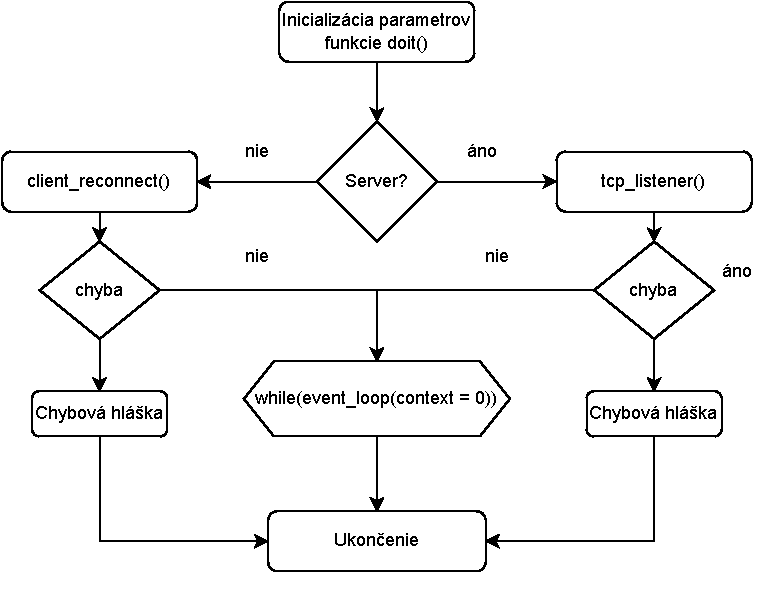
\includegraphics[width=0.9\textwidth]{figures/fc2}
	\caption{Princíp fungovania funkcie doit()}
	\label{fc2}
\end{figure}

\subsubsection{Funckia \lstinline|event_loop()|}
\lstinline|Event_loop()| je 111 riadkov dlhá funkcia. Jej obsah môžeme rozdeliť na overovací a výkonový. Úlohou niekoľkých \lstinline|if-ov| vo funkcii je preverovanie signálov, spätných hodnôt a podobných premenných, ktoré by signalizovali chybu, používateľov záujem o ukončenie programu alebo signál pre čítanie dát zo soketov, respektíve tunelov. 
 
Zaujímavé je taktiež predom definované makro \lstinline|BUFFERBLOAT_CONTROL|. Jeho úlohou je zamedzenie problému zvaného \textbf{Bufferbloat}. V skratke, je to nechcený jav, ktorý je zapríčinený nadmerným ukladaním paketov do vyrovnávacej pamäte, tzv. zahltenie. To ma za následok vysokú latenciu a tzv. z ang. \textit{Packet Delay Variation} (ďalej \acrshort{pdv}/Jitter), v paketovo-orientovaných sieťach. Viac o tejto problematike je možne si prečítať na \cite{bufferbloat}.
 
Na druhej strane výkonové funkcie, ako hovorí ich názov. niečo vykonávajú. Do tejto kategórie sme zaradili funkcie:
 \begin{itemize}
 	\item\lstinline|tcp_accept()| -- slúži na nastolenie nového soketového TCP spojenia s klientom, 
 	\item\lstinline|tun_read()| -- v prípade linuxového OS, volá \lstinline|safe_read_partial()| na zapísanie dát do nami vytvoreného tunelovacieho rozhrania,
 	\item\lstinline|uc_encrypt()| -- kryptografické šifrovanie paketov z tunelovacieho rozhrania,
 	\item\lstinline|safe_write_partial()| -- používa štandardizovanú funkciu \lstinline|write()| vo while cykle, zapíše zašifrované dáta do buffera určeného pre odoslanie klientovi, vracia počet zapísaných dát,
 	\item\lstinline|safe_write()| -- používa sa v prípade ak došlo k zahlteniu paketmi,
 	\item\lstinline|client_reconnect()| -- slúži na obnovu spojenia v prípade chyby,
 	\item\lstinline|safe_read_partial()| -- obdobne ako pri \lstinline|write()|, používa \lstinline|read()| funkciu,
 	\item\lstinline|uc_decrypt()| -- kryptografické dešifrovanie správy a následne odoslanie na tunelovacie rozhranie,
 	\item\lstinline|tun_write()| -- volá \lstinline|safe_write| pri OS Linux, teda klasický zápis dešifrovaných dát.
 \end{itemize}
Metóda použitá pri zápise zašifrovaných dát vo funkcii \lstinline|event_loop()| je znázornená v \ref{ed}.

 \begin{minipage}{\linewidth} 	
 	\begin{lstlisting}[frame=single,
 		numbers=left,
 		caption={Spôsob zápisu šifrovaných dát}\label{ed},
 		basicstyle=\ttfamily\small, keywordstyle=\color{black}\bfseries,]
 		
 writenb = safe_write_partial(context->client_fd, tun_buf.len,
 			    	 		         		  2U + TAG_LEN + len); 
 if (writenb < (ssize_t) 0) {// kontrola zahltenia -- bufferbloat
 	context->congestion = 1; 
 	writenb             = (ssize_t) 0;
 }
// ak doslo k zahlteniu
 if (writenb != (ssize_t)(2U + TAG_LEN + len)) {
 	writenb = safe_write(context->client_fd, tun_buf.len + writenb,
 	2U + TAG_LEN + len - writenb, TIMEOUT); 
 }
   	\end{lstlisting}
\end{minipage}\\ 
V princípe celá logika tejto VPN pozostáva z kontroly obsahu tunelovacieho rozhrania a aktívnych soketov. Následne ak sa na vstupoch nachádzajú dáta dochádza k ich čítaniu, dešifrovaniu a následnému odoslaniu dát aplikácií, ktorej prislúchajú.

Na konci funkcie \lstinline|event_loop()| sa nachádza ešte overenie pre prípad keď buffer s dátami nie je úplne plný. V tomto prípade funkcia vykonáva posun uložených bajtov na začiatok buffera. Inými slovami pripravuje dáta na ďalšie čítanie. Vyššie uvedené výroky sú znázornené v zdrojovom kóde \ref{bufferPreparation}.

\begin{lstlisting}[frame=single,
	numbers=left,
	caption={Príprava dát na ďalšie čítanie}\label{bufferPreparation},
	basicstyle=\ttfamily\small, keywordstyle=\color{black}\bfseries,]
	
	if (2 + TAG_LEN + MAX_PACKET_LEN != len_with_header) { 
		unsigned char *rbuf      = client_buf->len;
		size_t         remaining = client_buf->pos - len_with_header;
		memmove(rbuf, rbuf + len_with_header, remaining);
	}
	client_buf->pos -= len_with_header;
\end{lstlisting}
 
\subsubsection{Šifrovanie a dešifrovanie}
Proces šifrovanie resp. dešifrovania správy nastáva na oboch stranách spojenia, teda pri klientovi aj serveri. Zdrojový kód \ref{SS} demonštruje šifrovanie implementované v funkcii \lstinline|uc_encrypt()|. Tento proces sme sa pokúsili opísať v grafe \ref{fc3}. 

\begin{figure}
	\centering
	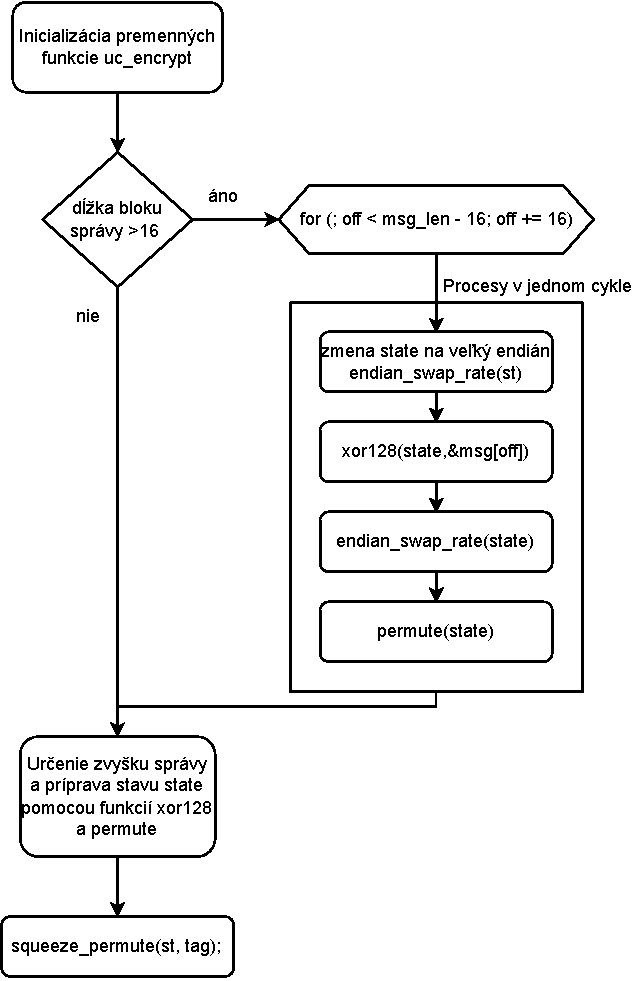
\includegraphics[width=0.7\textwidth]{figures/fc3}
	\caption{Proces šifrovania v funkcii uc\_encrypt()}
	\label{fc3}
\end{figure}

\begin{minipage}{\linewidth} 	
	\begin{lstlisting}[frame=single,
		numbers=left,
		caption={Šifrovanie správy pomocou uc\_encrypt}\label{SS},
		basicstyle=\ttfamily\small, keywordstyle=\color{black}\bfseries,]
 		
void uc_encrypt(uint32_t st[12], unsigned char *msg, 
					      size_t msg_len, unsigned char tag[16])
{	//spracovanie po 16 znakov
	unsigned char squeezed[16];
	unsigned char padded[16 + 1];
	size_t        off = 0;
	size_t        leftover;
	
	if (msg_len > 16) {
		for (; off < msg_len - 16; off += 16) {
			endian_swap_rate(st);
			memcpy(squeezed, st, 16);
			xor128(st, &msg[off]);
			endian_swap_rate(st);
			xor128(&msg[off], squeezed);
			permute(st);
		}
	}
	leftover = msg_len - off;
	memset(padded, 0, 16);
	mem_cpy(padded, &msg[off], leftover);
	padded[leftover] = 0x80;
	endian_swap_rate(st);
	memcpy(squeezed, st, 16);
	xor128(st, padded);
	endian_swap_rate(st);
	st[11] ^= (1UL << 24 | (uint32_t) leftover >> 4 << 25
				    | 1UL << 26); 
	xor128(padded, squeezed);
	mem_cpy(&msg[off], padded, leftover);
	permute(st);
	squeeze_permute(st, tag);		//vytvorenie tagu
}
  	\end{lstlisting}
\end{minipage}\\ 

Ako je viditeľne v kóde dochádza k častému použitiu 2 funkcií. Nimi sú  \lstinline|xor128()| a  \lstinline|permute()|. Jedná sa o pomerne dôležité bloky pre správne fungovanie šifrovacieho algoritmu. Obsah prvej z uvedených je preto znázornený v zdrojovom kóde \ref{xor}.

\begin{minipage}{\linewidth} 	
	\begin{lstlisting}[frame=single,
		numbers=left,
		caption={Funkcia xor128}\label{xor},
		basicstyle=\ttfamily\small, keywordstyle=\color{black}\bfseries,]
static inline void xor128(void *out, const void *in)
{
	#ifdef __SSSE3__
	_mm_storeu_si128((__m128i *) out,
	_mm_xor_si128(_mm_loadu_si128((const __m128i *) out),
	_mm_loadu_si128((const __m128i *) in)));
	#else
	unsigned char *      out_ = (unsigned char *) out;
	const unsigned char *in_  = (const unsigned char *) in;
	size_t               i;
	
	for (i = 0; i < 16; i++) {	//xororvanie jednotlivych znakov 
		out_[i] ^= in_[i];		//v 16 bitovom bloku spravy
	}
	#endif
}
  	\end{lstlisting}
\end{minipage}\\ 

Funkcia \lstinline|permute()| je pomerne rozsiahla. Jej obsah sa rozprestiera na 100 riadkoch. Jedná sa o implementáciu XOODOO permutácie, ktorá bola opísaná v kapitole číslo 2. Funkcionalita závisí od prostredia a procesorových inštrukcií. Samozrejmosťou je softvérová implementácia, ktorá je aj použitá pri behu. Dôvodom je, že naše zariadenie nemá k dispozícií uvedené procesorové inštrukcie. Blok, ktorý je použitý pri volaní sa nachádza v \ref{permute}.   

\begin{minipage}{\linewidth} 	
	\begin{lstlisting}[frame=single,
		numbers=left,
		caption={Funkcia Permute + makrá }\label{permute},
		basicstyle=\ttfamily\small, keywordstyle=\color{black}\bfseries,]
#define ROTR32(x, b) (uint32_t)(((x) >> (b)) | 
                     ((x) << (32 - (b))))
#define SWAP32(s, u, v)        \
do {                           \
	t      = (s)[u];             \
	(s)[u] = (s)[v], (s)[v] = t; \
} while (0)
	
static void permute(uint32_t st[12])
{
	uint32_t e[4], a, b, c, t, r, i;	
	for (r = 0; r < XOODOO_ROUNDS; r++) {
		for (i = 0; i < 4; i++) {
			e[i] = ROTR32(st[i] ^ st[i + 4] ^ st[i + 8], 18);
			e[i] ^= ROTR32(e[i], 9);
		}
		for (i = 0; i < 12; i++) {
			st[i] ^= e[(i - 1) & 3];
		}
		SWAP32(st, 7, 4);
		SWAP32(st, 7, 5);
		SWAP32(st, 7, 6);
		st[0] ^= RK[r];
		for (i = 0; i < 4; i++) {
			a         = st[i];
			b         = st[i + 4];
			c         = ROTR32(st[i + 8], 21);
			st[i + 8] = ROTR32((b & ~a) ^ c, 24);
			st[i + 4] = ROTR32((a & ~c) ^ b, 31);
			st[i] ^= c & ~b;
		}
		SWAP32(st, 8, 10);
		SWAP32(st, 9, 11);
	}	
}
	\end{lstlisting}
\end{minipage}\\
Na druhej strane k \textbf{dešifrovaniu} dochádza v momente ak sa v klientskom sokete nachádzajú dáta. Program overuje či sú v premennej \lstinline|fds[POLLFD_CLIENT]| dáta určené na spracovanie. \lstinline|fds[POLLFD_CLIENT]| predstavuje smerník na pamäťový blok, kde je uložený soket na druhú stranu spojenia, teda akceptovaného klienta. V momente keď sa tam nachádzajú dáta dôjde k ich čítaniu pomocou funkcie \lstinline|safe_read_partial()|. Následne program realizuje dešifrovanie funkciou \lstinline|uc_decrypt()|, ktorá je inverznou k \lstinline|uc_encrypt()|. V ukážke zdrojového kódu \ref{decrypt}, si používateľ môže prezrieť obsah funkcie \lstinline|uc_decrypt()|. Po odšifrovaní dát ich program zapisuje do tunelovacieho rozhrania prostredníctvom funkcie \lstinline|tun_write()|. Následne TUN rozhranie dotvára paket a vloží ho do sieťového zásobníka\footnote{z ang. \textit{network stack}}. OS následne vykonáva ďalšie spracovanie paketu do nižších vrstiev sieťového modelu. 

\begin{minipage}{\textwidth} 	
	\begin{lstlisting}[frame=single,
		numbers=left,
		caption={Funkcia Permute + makrá }\label{decrypt},
		basicstyle=\ttfamily\small, keywordstyle=\color{black}\bfseries,]
		int uc_decrypt(uint32_t st[12], unsigned char *msg, 
		               size_t msg_len, 
		               const unsigned char *expected_tag,
		               size_t expected_tag_len)
		{
			unsigned char tag[16];
			unsigned char squeezed[16];
			unsigned char padded[16 + 1];
			size_t        off = 0;
			size_t        leftover;
			
			if (msg_len > 16) {
				for (; off < msg_len - 16; off += 16) {
					endian_swap_rate(st);
					memcpy(squeezed, st, 16);
					xor128(&msg[off], squeezed);
					xor128(st, &msg[off]);
					endian_swap_rate(st);
					permute(st);
				}
			}
			leftover = msg_len - off;
			memset(padded, 0, 16);
			mem_cpy(padded, &msg[off], leftover);
			endian_swap_rate(st);
			memset(squeezed, 0, 16);
			mem_cpy(squeezed, 
			        (const unsigned char *) (const void *) st, 
			        leftover
			        );
			xor128(&padded, squeezed);
			padded[leftover] = 0x80;
			xor128(st, padded);
			endian_swap_rate(st);
			st[11] ^= (1UL << 24 | (uint32_t) leftover >> 4 
			           << 25 | 1UL << 26);
			mem_cpy(&msg[off], padded, leftover);
			permute(st);
			squeeze_permute(st, tag);
			\\
			if (equals(expected_tag, tag, expected_tag_len) == 0) {
				memset(msg, 0, msg_len);
				return -1;
			}
			return 0;
		}
	\end{lstlisting}
\end{minipage}\\




Pre čitateľa sme si pripravili aj názornú ukážku šifrovania a prenosu týchto dát cez soket. Za účelom ukážky použijeme už spomínaný nástroj Wireshark na zachytávanie premávky v sieťových rozhraniach. Prechod dát z pohľadu klienta medzi zariadeniami je znázornený na obrázku \ref{wiresharkpakety}. 
% TODO: \usepackage{graphicx} required
\begin{figure}[h!]
	\centering
	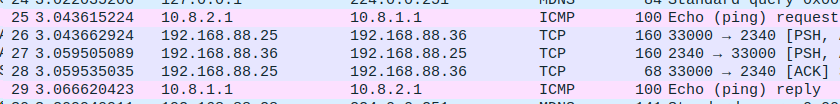
\includegraphics[width=1\textwidth]{figures/wiresharkpakety}
	\caption{Prenos zašifrovaných dát z VPN klienta na VPN server}
	\label{:wiresharkpakety}
\end{figure}
Na VPN klientovi sme spustili v príkazovom riadku jednoduchý príkaz \lstinline|ping 10.8.1.1|. Ten nám vytvára veľmi známy ICMP paket so žiadosťou o odpoveď\footnote{paket číslo 25}. Obsah tohto paketu je možné si pozrieť v obrázku \ref{req}. % TODO: \usepackage{graphicx} required
\begin{figure}[h!]
	\centering
	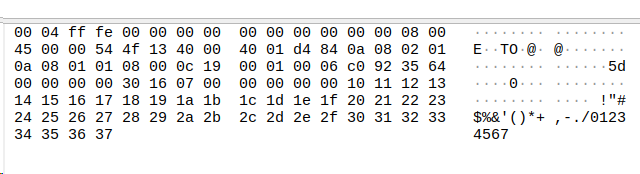
\includegraphics[width=1\textwidth]{figures/req}
	\caption{Obsah pôvodného paketu s ICMP žiadosťou}
	\label{req}
\end{figure}
Tento paket je vo VPN klinetovi po spracovaní vo DSVPN zašifrovaný pomocou XOODOO permutácie a odoslaný cez soketové TCP spojenie\footnote{paket číslo 26}. Obsah zašifrovaného paketu je znázornený v \ref{sifrovanypaket}. 
% TODO: \usepackage{graphicx} required
\begin{figure}[h!]
	\centering
	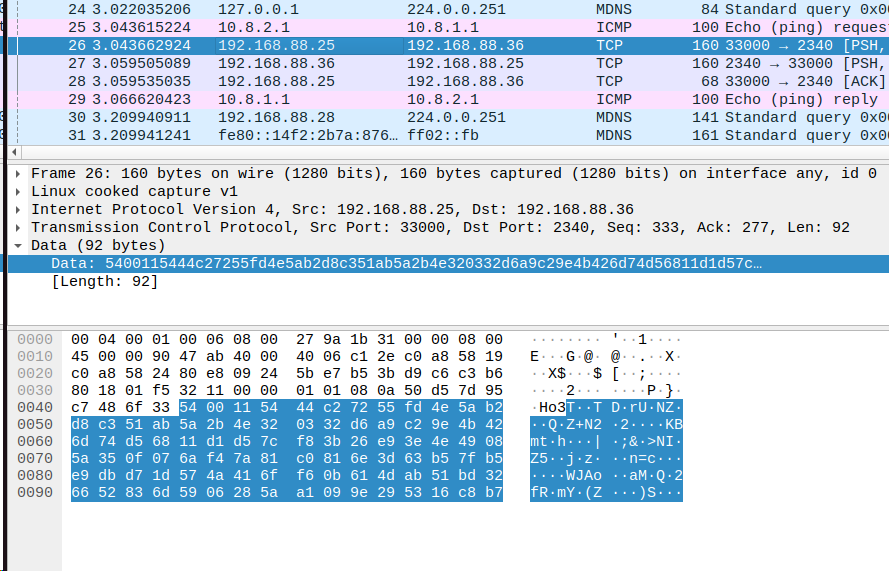
\includegraphics[width=0.9\textwidth]{figures/sifrovanypaket}
	\caption{Zašifrovaný pôvodný ICMP paket v novom TCP pakete}
	\label{sifrovanypaket}
\end{figure}
Označená časť paketu v obrázku je už spomenutý zašifrovaný ICMP paket z obrázku \ref{req}. VPN server ho po prijatí dešifruje a posiela na vlastné tunelovacie rozhranie. Odiaľ prevezme paket OS a vygeneruje odpoveď na pôvodnú požiadavku vo forme nového paketu. Ten je prenesený na klienta opäť cez soketové TCP spojenie\footnote{paket číslo 27}. Paket číslo 28 je odpoveď na úspešne prijatie. DSVPN spracuje tento paket a zapíše pôvodný na tunelovacie rozhranie.. Z hľadiska klienta už vidíme dešifrovanú odpoveď v pakete číslo 29, ktorú spracuje OS.

  
\subsubsection{Ukončenie činnosti programu}
Používateľ má možnosť ukončiť vzniknuté VPN spojenie medzi klientom a serverom pomocou jednoduchého príkazu \lstinline|crtl + c|. Program zaznamená tento vstup a ukončí cyklus. Po návrate až do hlavnej funckie \lstinline|main()| sa z OS vymažú aplikované FW pravidlá a používateľ môže používať počítač ako pred spustením DSVPN.

\section{Analýza výpočtových nárokov DSVPN}\label{analyza}
Za účelom analýzy výpočtových nárokov sme sa v práci zamerali na meranie potrebného počtu cyklov a zároveň aj času, potrebného na vykonanie šifrovanie a dešifrovanie permutacie XOODOO. Pre linuxovú platformu sme použili niektoré zabudované funkcie ako je \lstinline|clock()|. Pomocou nej sme zmerali čas vykonávania. Ukážka ako bol kód na meranie implementovaný do DSVPN je možné vidieť v ukážke zdrojového kódu
 
\begin{minipage}{\linewidth} 	
	\begin{lstlisting}[frame=single,
		numbers=left,
		caption={Ukážka spôsobu merania pri (de)šifrovaní XOODOO}\label{mneranie},
		basicstyle=\ttfamily\small, keywordstyle=\color{black}\bfseries,]
		uint64_t time,tick;	//inicializacia premennych
		clock_t t = clock();
		
		tick = cpucyclesS();
		codeTomeassure();		//funkcia urcena na meranie
		time = cpucyclesE()-tick;
		
		t = clock() - t;    //vyhodnotenie
		double time_taken = ((double)t)/CLOCKS_PER_SEC;
		printf(Size(%ld B): "%llu cycles in %f s\n", msg_length,
		       time, time_taken);	
	\end{lstlisting}
\end{minipage}\\
V prípade, ak by používateľ potreboval vykonať podobné meranie času v prostredí OS Windows, tak dávame do pozornosti tento variant. Viď zdrojový kód \ref{winmer}. Viac o použití a limitáciách je možné nájsť v práci \cite{bc}.

\begin{minipage}{\linewidth} 	
	\begin{lstlisting}[frame=single,
		numbers=left,
		caption={Meranie času vykonávania na OS Windows}\label{winmer},
		basicstyle=\ttfamily\small, keywordstyle=\color{black}\bfseries,]
	#include <windows.h>
	
	#define TIMER_INIT \	//inicializacia makra
	LARGE_INTEGER frequency; \
	LARGE_INTEGER t1,t2; \
	double elapsedTime; \
	QueryPerformanceFrequency(&frequency);

	#define TIMER_START QueryPerformanceCounter(&t1);
	#define TIMER_STOP \
	QueryPerformanceCounter(&t2); \
	elapsedTime=(double)(t2.QuadPart-t1.QuadPart)
						  /frequency.QuadPart; 	
	
	TIMER_INIT		\\pouzitie	
	{
		TIMER_START
		codeToMeasure()
	 	TIMER_STOP
 	}
	\end{lstlisting}
\end{minipage}\\

Spojenie medzi klientom a serverom je spustené na VM. Šifrovanie bolo merané na strane Klienta. Dešifrovanie sme merali v OS servera. Počas spojenia sme sa snažili naviesť stav väčšieho sieťového zataženia. Tento úkon sme zrealizovali otvorením viacerých rôznych kariet vo webovom prehliadači. Týmto spôsobom sme odsimuloval potrebu prenosu vačšieho množstva dát naprieč sieťou. Najčastejšie však do šifrovania vstupovali TCP pakety, ktoré majú za úlohu udržať soketové TCP spojenie. Ich veľkosť je 52bajtov. Z výpisu sme ešte na základe pozorovania sledovali aké veľkosti sa najčastejšie vyskytujú. Na základe takto získaných dát sme vypracovali tabuľku \ref{tabmer}. Hodnoty pre jednotlivé stĺpce boli získane ako aritmetický priemer z meraní. Pakety, ktoré vstupovali do šifrovania, resp. dešifrovania menej ako 20-krát sme z meraní vypustili. Dôvodom je snaha o získanie lepších štatistických údajov. Obdobne sme pri výpočte aritmetického priemeru nebrali do úvahy príliš veľké výchylky pri meraní počtu cyklov. Uvedené chyby merania spôsobil samotný OS, kvôli prerušovania činnosti programu DSVPN.     

\begin{table}[h!]
	\centering
	\resizebox{\textwidth}{!}{%
		\begin{tabular}{c|c|c|c|c}
			\bfseries Veľkosť dát[B] &
			\multicolumn{4}{|c}{\bfseries Názov meranej funkcie} 			
			\\
			\bfseries X &
			\multicolumn{2}{|c}{\bfseries uc\_encrypt()} &
			\multicolumn{2}{|c}{\bfseries uc\_decrypt()}
			\\
			\bfseries Počet meraní 
			& Počet cyklov
			& Čas vykonávania [s]
			& Počet cyklov
			& Čas vykonávania [s] 
			\\\hline\hline
			 52   X 1376			 
			& 1 648
			& 0.000 076
			& 2 377
			& 0.000 062
			\\		
			60  X  79	
			& 2 527
			& 0.000 049
			& 2 769
			& 0.000 044
			\\	
			64 X 47		
			& 1 799
			& 0.000 048
			& 2 341
			& 0.000 043
			\\
			 80  X 145		
			& 2 853
			& 0.000 053
			& 3 343
			& 0.000 057
			\\ 
			 91  X 128		
			& 2 944
			& 0.000 046
			& 2 965
			& 0.000 042
			\\
			116 X 35		
			& 4 083
			& 0.000 049
			& 2 878
			& 0.000 049
			\\
			222 X 23		
			& 4 220
			& 0.000 345
			& 3 976
			& 0.000 040
			\\
			569 X 51		
			& 10 245
			& 0.000 950
			& 8 574
			& 0.000 043
			\\
			1 385 X 147		
			& 21 232
			& 0.000 165
			& 19 046
			& 0.000 045
			\\
			1 452 X 14		
			& 22 599
			& 0.000 077
			& 20 083
			& 0.000 532
			\\\hline\hline
		 	\bfseries	Celkom [B]		
			& -
			& -
			& -
			& - 
			\\
			364 656		
			& 74 150
			& 0.001 858
			& 68 352
			& 0.000 957
						
		\end{tabular}%
	}
	\caption{Výsledky získaných meraní}
	\label{tabmer}
\end{table}
Ako môžeme vidieť z experimentálnych meraní, tak implementácia XOODOO algoritmu je na bežnom počítači extrémne rýchla. Faktom ostáva že do meraní nám vo veľkej miere zásahuje OS. Okrem tohto faktu bežal klient aj server vo virtuálnom prostredí nad iným natívnym OS, so značne obmedzeným výkonom. Z výsledkov však môžeme zhodnotiť, že šifrovanie a dešifrovanie dokáže držať na úrovní 40-70 mikrosekúnd v závislosti od veľkosti vstupujúcich dát a prostredia, na ktorom aplikácia beží.

Súčasťou príloh sú súbory s logmi, z ktorých bola tabuľka vytvorená. Zároveň prikladáme aj zdrojový kód programu, ktorý bol použitý na spracovanie výsledkov. Viď priečinok \lstinline|Measurements|. 
\section{Windows kompatibilita}

% !TEX root = ../thesis.tex
\chapter{Vyhodnotenie dosiahnutých výsledkov}
V rámci tejto kapitoly zhrnieme dosiahnuté výsledky z analýzy, experimentálnych meraní a rozšírenia kompatibility pre OS Windows.
\section{Analýza jednoduchej VPN siete}
V úvode praktickej časti sme postupnou analýzou prešli jednotlivé časti zdrojového kódu DSVPN. Názorne sme opisovali dôležité bloky a funkcionalitu implementovanú v tejto jednoduchej VPN. Na základe nadobudnutých znalostí sme vypracovali stavové diagramy, ktoré čitateľovi jednoznačne vysvetľujú čo sa v programe realizuje. Na základe týchto informácií, dokáže pochopiť ako sa v praxi realizuje VPN sieťové spojenie.
\section{Experimentálne meranie autentizovaného šifrovania pomocou permutácie XOODOO}
Popri analýze zdrojového kódu sme experimentálne overili funkcionalitu autentizovaného šifrovania pomocou permutácie XOODOO v jednoduchej VPN sieti.  Simuláciu bežného prostredia sme uskutočnili za pomoci 2 virtuálnych OS a~jedného natívneho OS, na ktorom virtuálizácia prebiehala. Virtualizované zariadenia mali obdobne aj obmedzený výpočtový výkon a pridelené prostriedky. To sa prejavovalo v pomalších odozvách systémov na požiadavky používateľa. 

Zo získaných výsledkov v tabuľke \ref{tabmer} sme usúdili, že virtuálne prostredie nie je vhodné pre meranie. Z toho dôvodu sme vytvorili program, ktorý používa kryptografické funkcie z implementácie DSVPN. XOODOO permutáciu sme inicializovali podľa vzoru v DSVPN. Následne sme vygenerovali náhodné dáta a tie sme zašifrovali a dešifrovali. Získané dáta sú znázornené v~tabuľke~\ref{tabmerlokal}. 

\begin{table}[h!]
	\centering
	\resizebox{\textwidth}{!}{%
		\begin{tabular}{c|c|c|c|c}
			\multirow{2}{*}{\bfseries Veľkosť dát [B]} &
			\multicolumn{2}{|c}{\bfseries uc\_encrypt()} &
			\multicolumn{2}{|c}{\bfseries uc\_decrypt()} 
			\\
			& Počet cyklov
			& Čas vykonávania [ms]
			& Počet cyklov
			& Čas vykonávania [ms] 
			\\\hline\hline
			52		 
			& 15 428
			& 0,005 600
			& 16 124
			& 0,005 700
			\\		
			250
			& 50 634
			& 0,017 600
			& 50 866
			& 0,017 700
			\\	
			500		
			& 97 817
			& 0,034 000
			& 97 469
			& 0,033 800
			\\
			1 000		
			& 189 312
			& 0,065 600
			& 189 167
			& 0,065 500
			\\ 
			1 500		
			& 280 691
			& 0,097 100
			& 280 749
			& 0,097 100
			\\
			3 000		
			& 557 322
			& 0,192 700
			& 557 960
			& 0,192 900
			\\
			4 500		
			& 834 997
			& 0,288 600
			& 835 374
			& 0,288 700
			\\
			6 000		
			& 1 110 120
			& 0,383 600
			& 1 109 279
			& 0,383 300
			\\
			7 500		
			& 1 397 974
			& 0,483 100
			& 1 386 258
			& 0,479 000
			\\
			9 000		
			& 1 769 841
			& 0,611 600
			& 1 661 352
			& 0,574 100			
		\end{tabular}%
	}
	\caption{Výsledky z experimentálnych meraní funkcií na šifrovanie a dešifrovanie v prostredí lokálneho zariadenia}
	\label{tabmerlokal}
\end{table} 
Z týchto výsledkov už je jednoznačne, že čas vykonávania šifrovania a dešifrovania, je priamo úmerný veľkosti dát vstupujúcich do XOODOO permutácie. To isté platí aj pre počet vykonaných cyklov. Rádovo sa čas vykonávania počas merania pohyboval pod úrovňou 1 milisekundy a to aj pri šifrovaní dát o veľkosti 9000 bajtov, ktorá predstavuje maximálnu možnú prenosovú veľkosť paketu (MTU). To znamená, že v implementácií DSVPN do (de)šifrovania nevstupujú väčšie dáta. Použitie permutácie XOODOO na zariadení je teda extrémne rýchle a jej použitie pri sieťovom prenose je z používateľského hľadiska zanedbateľné. 

Vytvorený zdrojový kód na meranie šifrovania a dešifrovania je obsahom Prílohy A.4. Konkrétne v priečinku \lstinline|MeasurementsInLocalEnvironment|.
    
\section{Výsledky dosiahnuté pri tvorbe kompatibility \\DSVPN pre OS Windows}
Jedným z cieľov našej práce bolo aj rozšírenie pôvodného riešenia DSVPN o~kompatibilitu pre OS Windows. Samozrejmosťou bolo zachovanie pôvodnej kompatibility v rámci ostatných OS. V princípe sa nám podarilo vytvoriť tunelové spojenie medzi VPN klientom a VPN serverom so zabezpečeným prenosom dát. Taktiež je možné nadviazať spojenie nie len medzi zariadeniami s OS Windows, ale vieme spojiť ľubovoľné OS z množiny podporovaných DSVPN.  

Problém riešenia nastáva pri smerovaní paketov naspäť k pôvodnému vlastníkovi. Pomocou sieťových príkazov a monitoringu premávky sa nám nepodarilo doteraz zistiť, prečo sa odpoveď na pôvodnú požiadavku nedokáže vrátiť na~zariadenie. Tento úkon sa deje aj napriek tomu, že pri monitoringu vidíme ako paket s odpoveďou opúšťa zariadenie a prichádza na to, ktoré má dostať odpoveď. Súčasná hypotéza je, že nám uniká niečo pri smerovaní paketu z pozície OS Windows. Tento problém sa budeme snažiť ešte v blízkej budúcnosti vyriešiť, nakoľko by sa nemalo jednať o veľký problém. Čitateľ bude mať prístup ku aktuálnemu kódu pomocou stránky github.   
% !TEX root = ../thesis.tex

\chapter{Záver}
\label{summary}
Cieľom našej práce bolo uvedenie čitateľa do problematiky VPN sietí, so zameraním na použitie kryptografického algoritmu XOODOO permutácie za účelom zabezpečenia komunikácie. V~prvej časti práci sme zadefinovali potrebné pojmy spojené s problematikou VPN sietí. Následne sme postupným opisom charakterizovali čo sa deje v~sieťach typu VPN. Na základe naštudovanej literatúry sme vytvorili klasifikácie VPN sietí. Rozdelenie bolo realizované podľa logickej topológie a dát vstupujúcich do~šifrovania. Pomocou nadobudnutých informácií sme charakterizovali a špecifikovali činnosti implementované v známych VPN protokoloch. V závere prvej kapitoly sme zhrnuli rozdelenie VPN sietí pomocou grafu.

Druhá kapitola sa venuje problematike ľahkej kryptografie. V nej sme charakterizovali tento pomerné nový odbor v oblasti kryptografie. Následne sme pokračovali s opisom XOODOO permutácie, ktorú zaraďujeme do tejto kategórie. XOODOO permutácia je súčasťou kryptografického balíka Xoodyak, ktorý je jedným z finalistov štandardizačného procesu NIST v ľahkej kryptografie. Opísali sme činnosti v algoritme a vysvetlili možnosti použitia. 

Tretia kapitola obsahuje postupy prípravy prostredí na experimentovanie. Konfiguráciu virtualizovaných OS a opis jednotlivých nástrojov, ktoré boli pri práci použité. Opísali sme Wintun adaptér na tvorbu virtuálnych tunelovacích rozhraní v OS Windows. Za účelom použitia pri výučbe v špecializovaných predmetoch orientovaných na bezpečnost v počítačových sieťach, sme vytvorili jednoduché demo, ktoré demonštruje odosielanie a prijímanie ICMP paketov pomocou tohto adaptéru.

Štvrtá kapitola sa zameriava na praktickú demonštráciu jednoduchej VPN siete s využitím XOODOO permutácie. V úvode sme charakterizovali program DSVPN. Následne sme praktickým experimentom overili jeho funkčnosť. Z tejto činnosti sme vypracovali článok do Zborníka vedeckých prác TUKE FEI \cite{clanok}. Podrobne sme analyzovali zdrojový kód DSVPN. Popri analýze sme názorným spôsobom ukázali čo sa deje s paketmi. Experimentálne sme zmerali rýchlosť a počet cyklov implementácie XOODOO permutácie v DSVPN. Súčasťou našej práce bolo aj vytvorenie kompatibility DSVPN o OS Windows a opis vykonaných zmien. 

V piatej kapitole sme zhrnuli dosiahnuté výsledky z praktickej časti práce. Celý obsah prílohy A vrátane samotnej práce sme uverejnili na git stránku Github pod profilom mr171hg\footnote{\url{https://github.com/mr171hg/DiplomaProject}}. Dôvodom je dostupnosť týchto informácií pre každého, kto sa potrebuje v problematike VPN zorientovať.  

Výsledná podoba práce spoločne s demonštratívnymi príkladmi zdrojových kódov a ostatnými prílohami boli spracované tak, aby bolo možné ich použitie v~špecializovaných predmetoch zameraných na bezpečnosť v počítačových sieťach.

Pre účely rozšírenia práce by sme navrhovali pokračovať v práci na kompatibilite DSVPN. Rozšíriť implementáciu o viacero kryptografických algoritmov a následne experimentálne merať. Aplikovať program DSVPN na sieťové zariadenie a vyskúšať reálnu prevádzku. Refaktorovať a optimalizovať zdrojový kód. Rozšíriť program o možnosti pripojenia viacerých klientov na jeden server s využitím paralelného programovania s viac vláknami. 


% good linebraking of bibtex url
\setcounter{biburllcpenalty}{7000}
\setcounter{biburlucpenalty}{8000}

%% The bibliography
\printbibliography[heading=bibintoc]

\label{theend} % the last page of the thesis

% List of acronyms

% Glossaries
%\printglossary

%% Appendix
% !TEX root = ../thesis.tex

\chapter*{Zoznam príloh}
\addcontentsline{toc}{chapter}{Zoznam príloh}

\begin{description}
    \item[Príloha A] CD médium -- viď. obsah CD média
\end{description}


\appendix 
\renewcommand\chaptername{Príloha}
% !TEX root = ../thesis.tex

\chapter{Obsah CD Média} 

Prílohy v CD médiu sme rozdelili na tieto 4 časti:

\begin{itemize}
	\item \textbf{Príloha A.1} -- Zdrojové kódy referenčnej implementácie XOODOO spoločne s kódom na otestovanie správnosti algoritmu Xoocycle 
	\item\textbf{Príloha A.2} -- Zdrojový kód s demo použítím Wintun adaptéra 
	\item \textbf{Príloha A.3} -- Zdrojový kód pôvodnej a rozšírenej DSVPN implementácie
	\item \textbf{Príloha A.4} -- Výsledky experimentálnych meraní spoločne so zdrojovými kódmi použitých programov 
\end{itemize}

Obsah celej tejto práce je dostupný na gite:
\begin{itemize}
	\item \url{https://github.com/mr171hg/DiplomaProject}
\end{itemize}

Obsah CD média je možné nájsť na stránke:
\begin{itemize}
	\item \url{https://github.com/mr171hg/DiplomaProject/tree/main/DiplomaWork/appendixes/Attachments}
\end{itemize}


% zivotopis autora
%\curriculumvitae\protect
%Táto časť\/ je nepovinná. Autor tu môže uviesť\/ svoje biografické
%údaje, údaje o~záujmoch, účasti na~projektoch, účasti na~súťažiach,
%získané ocenenia, zahraničné pobyty na~praxi, domácu prax, publikácie
%a~pod.

\end{document}
